
\newpage
\appendix

\section{反向传播算法}

\subsection{多层感知机反向传播}\label{sec:mlpbp}

在多层感知机(MLP)中,我们令网络共有 $L$ 层,第 $l$ 层的参数为权重矩阵 $W^{(l)}$ 和偏置向量 $b^{(l)}$。对于输入样本 $(x,y)$,定义:
\[
\begin{aligned}
&z^{(l)} = W^{(l)}\,a^{(l-1)} + b^{(l)},\quad
a^{(l)} = \sigma\bigl(z^{(l)}\bigr),\quad
a^{(0)} = x,\\
&\text{网络输出:}\;\hat y = a^{(L)},\quad
\text{损失函数:}\;L\bigl(\hat y,y\bigr)\,.
\end{aligned}
\]
其中:
- $x\in\mathbb R^{n_0}$:输入向量;
- $a^{(l)}\in\mathbb R^{n_l}$:第 $l$ 层的激活值,$n_l$ 为第 $l$ 层神经元数;
- $W^{(l)}\in\mathbb R^{n_l\times n_{l-1}}$,$b^{(l)}\in\mathbb R^{n_l}$:第 $l$ 层的权重和偏置;
- $\sigma(\cdot)$:激活函数(如 Sigmoid、ReLU 等);
- $L(\hat y,y)$:样本的损失,例如均方误差 $\tfrac12\|\hat y-y\|^2$ 或交叉熵。

\paragraph{误差项的定义}  
令第 $l$ 层的误差项(\emph{delta})为
\[
\delta^{(l)} \;=\;\frac{\partial L}{\partial z^{(l)}}
\;=\;\frac{\partial L}{\partial a^{(l)}}\;\odot\;\sigma'\bigl(z^{(l)}\bigr)\,,
\]
其中 $\odot$ 表示按元素乘,$\sigma'$ 是激活函数的导数。

\paragraph{向后传播}  
\begin{align}
&\text{输出层 }\;l=L:\quad
\delta^{(L)} = \bigl(a^{(L)} - y\bigr)\;\odot\;\sigma'\bigl(z^{(L)}\bigr)\,.\\
&\text{中间层 }\;l=L-1,\dots,1:\quad
\delta^{(l)} = \bigl(W^{(l+1)\,T}\,\delta^{(l+1)}\bigr)\;\odot\;\sigma'\bigl(z^{(l)}\bigr)\,.
\end{align}

\paragraph{梯度计算}  
对于每一层参数,梯度为
\[
\frac{\partial L}{\partial W^{(l)}} = \delta^{(l)}\,a^{(l-1)\,T},\quad
\frac{\partial L}{\partial b^{(l)}} = \delta^{(l)}\,.
\]

\paragraph{参数更新}  
使用梯度下降(学习率 $\eta>0$)更新:
\[
W^{(l)} \leftarrow W^{(l)} - \eta\,\frac{\partial L}{\partial W^{(l)}},\quad
b^{(l)} \leftarrow b^{(l)} - \eta\,\frac{\partial L}{\partial b^{(l)}}\,.
\]

---

\subsection{卷积神经网络反向传播}

在卷积层中,输入为多通道特征图 $a^{(l-1)}\in\mathbb R^{C_{in}\times H_{in}\times W_{in}}$,卷积核为 $W^{(l)}\in\mathbb R^{C_{out}\times C_{in}\times k_h\times k_w}$,偏置 $b^{(l)}\in\mathbb R^{C_{out}}$。前向传播:
\[
z^{(l)}_{c_o}(i,j)
=\sum_{c_i=1}^{C_{in}}\sum_{u=1}^{k_h}\sum_{v=1}^{k_w}
W^{(l)}_{c_o,c_i,u,v}\;a^{(l-1)}_{c_i}\bigl(i+u-1,\;j+v-1\bigr)
\;+\;b^{(l)}_{c_o},
\]
\[
a^{(l)} = \sigma\bigl(z^{(l)}\bigr)\,.
\]

\paragraph{误差项}  
设 \(\delta^{(l)} = \tfrac{\partial L}{\partial z^{(l)}}\in\mathbb R^{C_{out}\times H_{out}\times W_{out}}\)。

\paragraph{卷积核梯度}  
\[
\frac{\partial L}{\partial W^{(l)}_{c_o,c_i,u,v}}
=\sum_{i,j}\;
\delta^{(l)}_{c_o}(i,j)\;\cdot\;
a^{(l-1)}_{c_i}\bigl(i+u-1,j+v-1\bigr)\,,
\]
\[
\frac{\partial L}{\partial b^{(l)}_{c_o}}
=\sum_{i,j}\delta^{(l)}_{c_o}(i,j)\,.
\]

\paragraph{梯度反传到上一层特征图}  
\[
\frac{\partial L}{\partial a^{(l-1)}_{c_i}(x,y)}
=\sum_{c_o=1}^{C_{out}}\sum_{u=1}^{k_h}\sum_{v=1}^{k_w}
W^{(l)}_{c_o,c_i,u,v}\;
\delta^{(l)}_{c_o}\bigl(x-u+1,\;y-v+1\bigr)\,,
\]
即对卷积核翻转并“全卷积”(full convolution)。

\paragraph{池化层梯度}  
- \emph{最大池化}:将上层 $\delta$ 中的位置梯度“路由”回最大值位置,其余位置置零。  
- \emph{平均池化}:将上层 $\delta$ 按均匀分布「反池化」回每个位置。

\paragraph{参数更新}  
同 MLP,中使用学习率 $\eta$:
\[
W^{(l)} \leftarrow W^{(l)} - \eta\,\frac{\partial L}{\partial W^{(l)}},\quad
b^{(l)} \leftarrow b^{(l)} - \eta\,\frac{\partial L}{\partial b^{(l)}}\,.
\]



\section{tsne降维展示特征空间实验结果}\label{sec:hidden}
\begin{figure}[H]
    \centering
    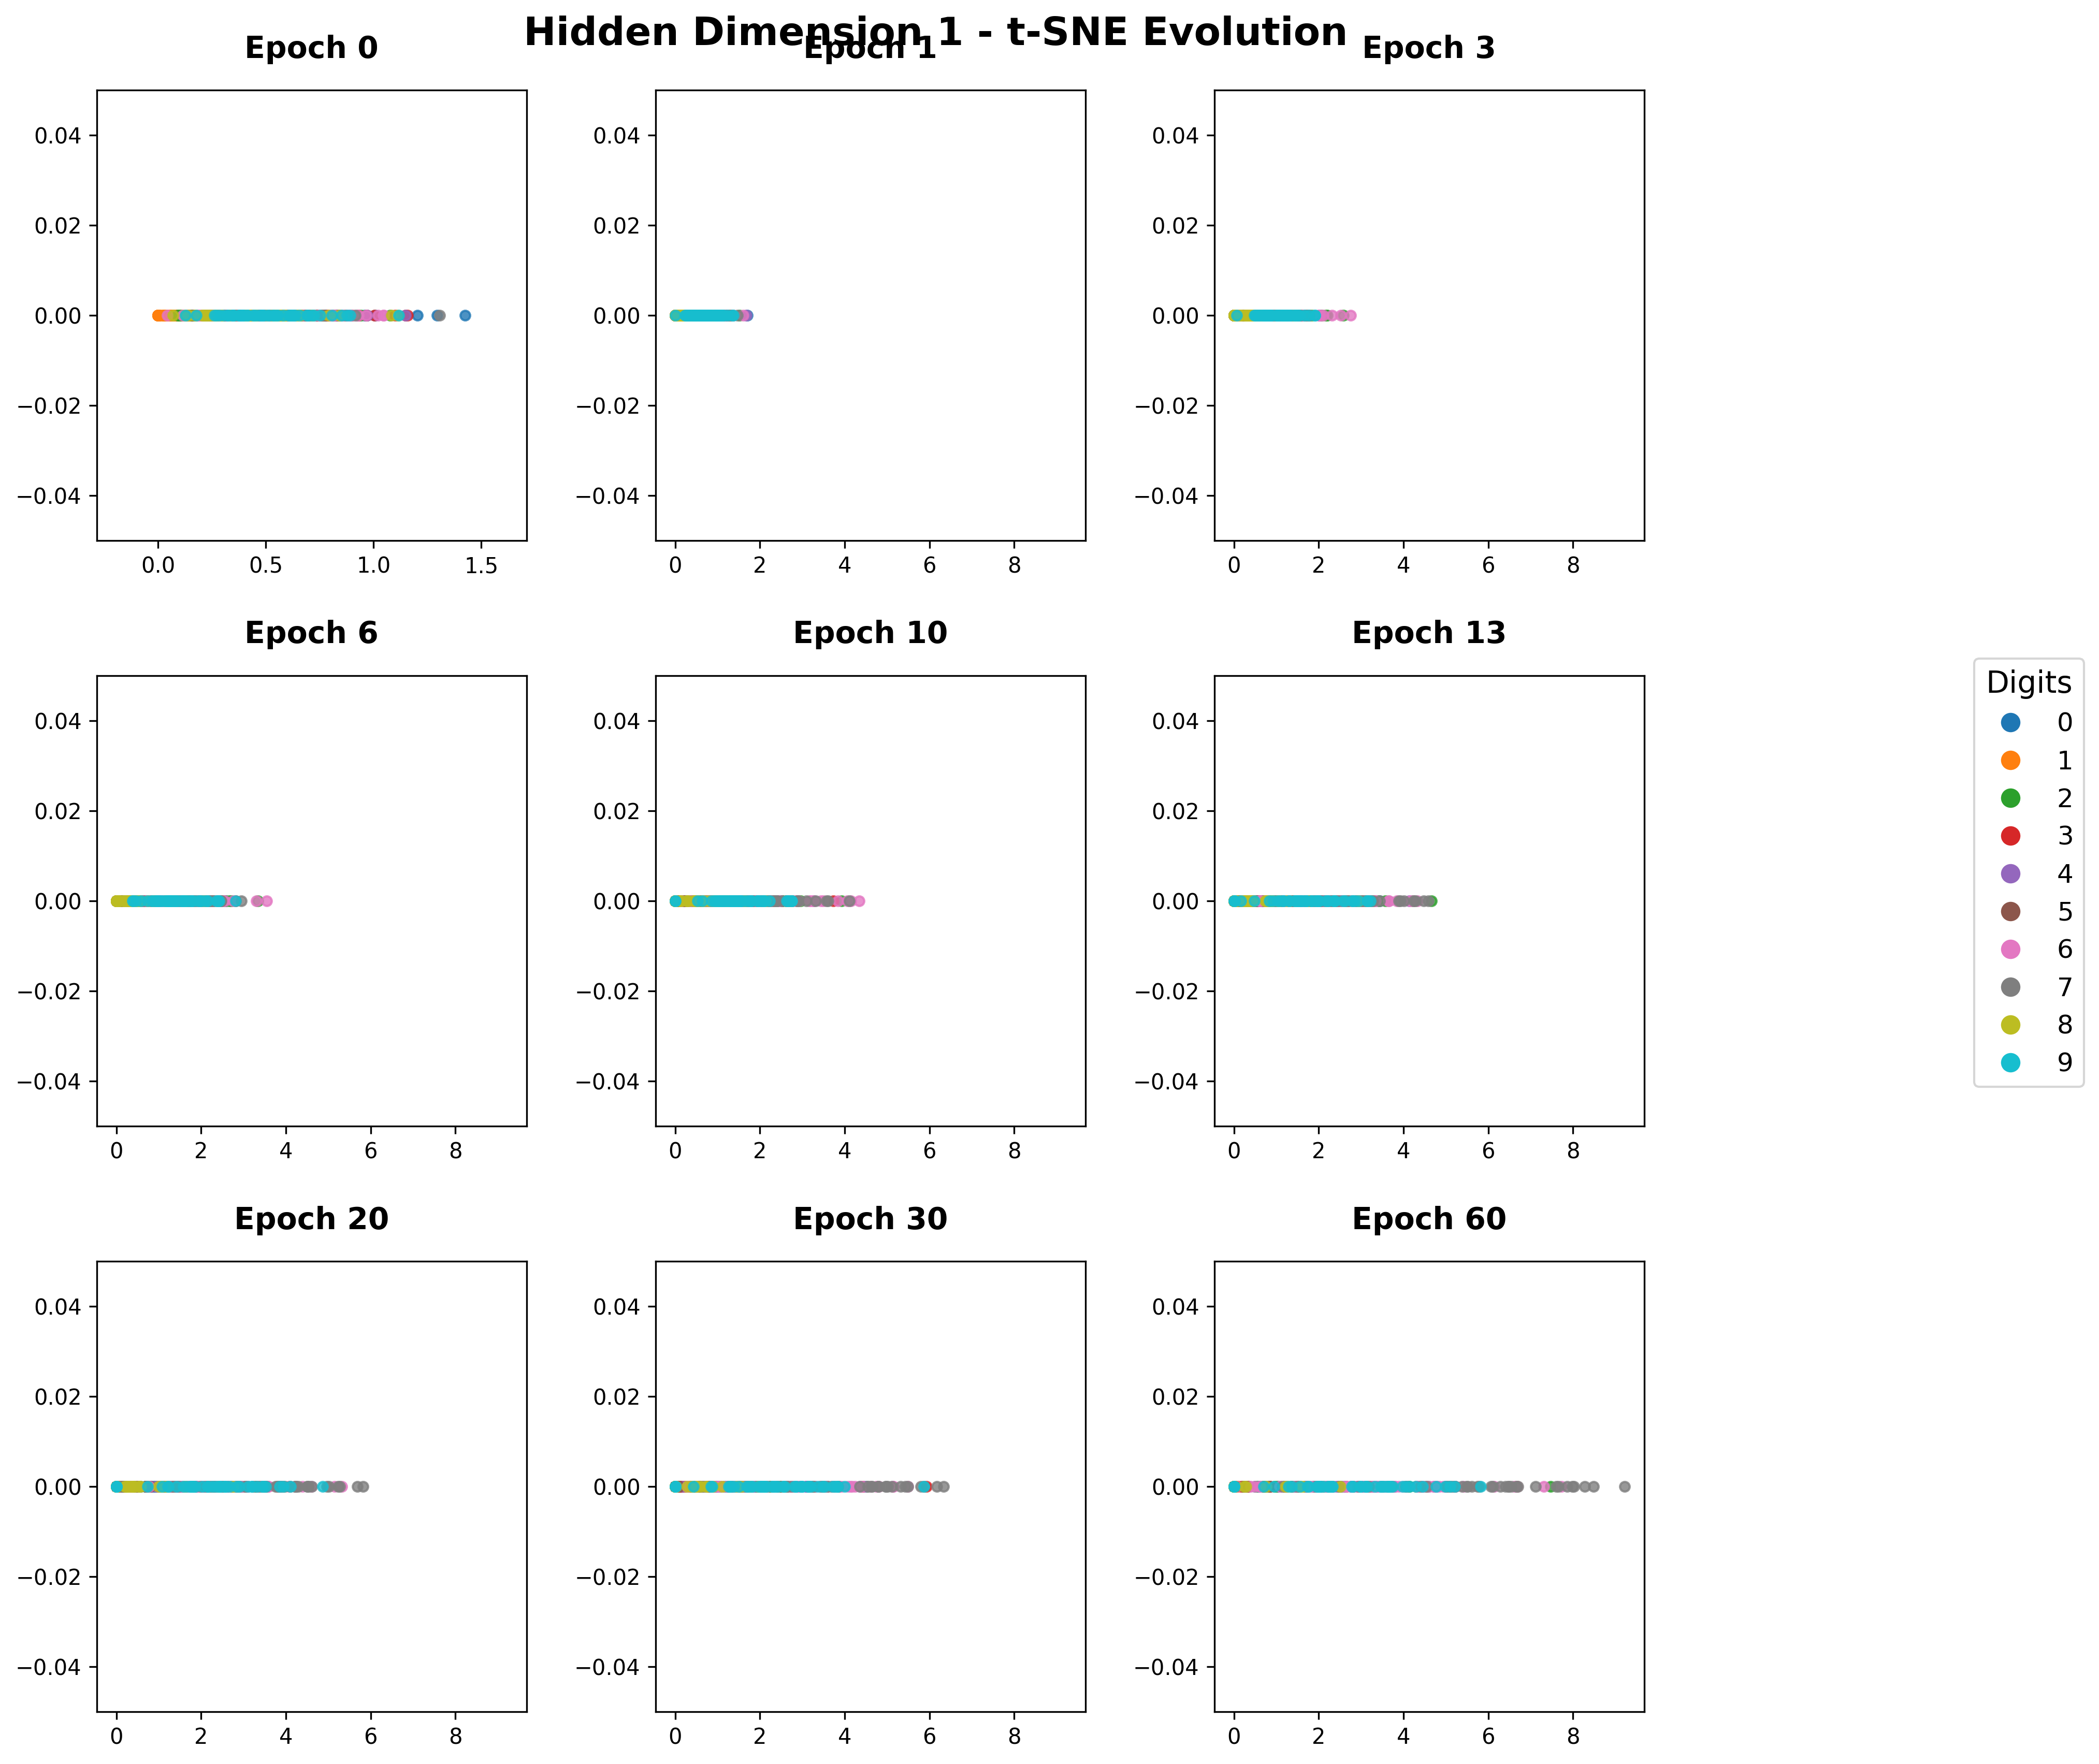
\includegraphics[width=0.8\textwidth]{../images/pa/tsne_evolution_hidden_1.png}
    \caption{隐层神经元数为1时的t-SNE可视化演化}
    \label{fig:1}
\end{figure}
\begin{figure}[H]
    \centering
    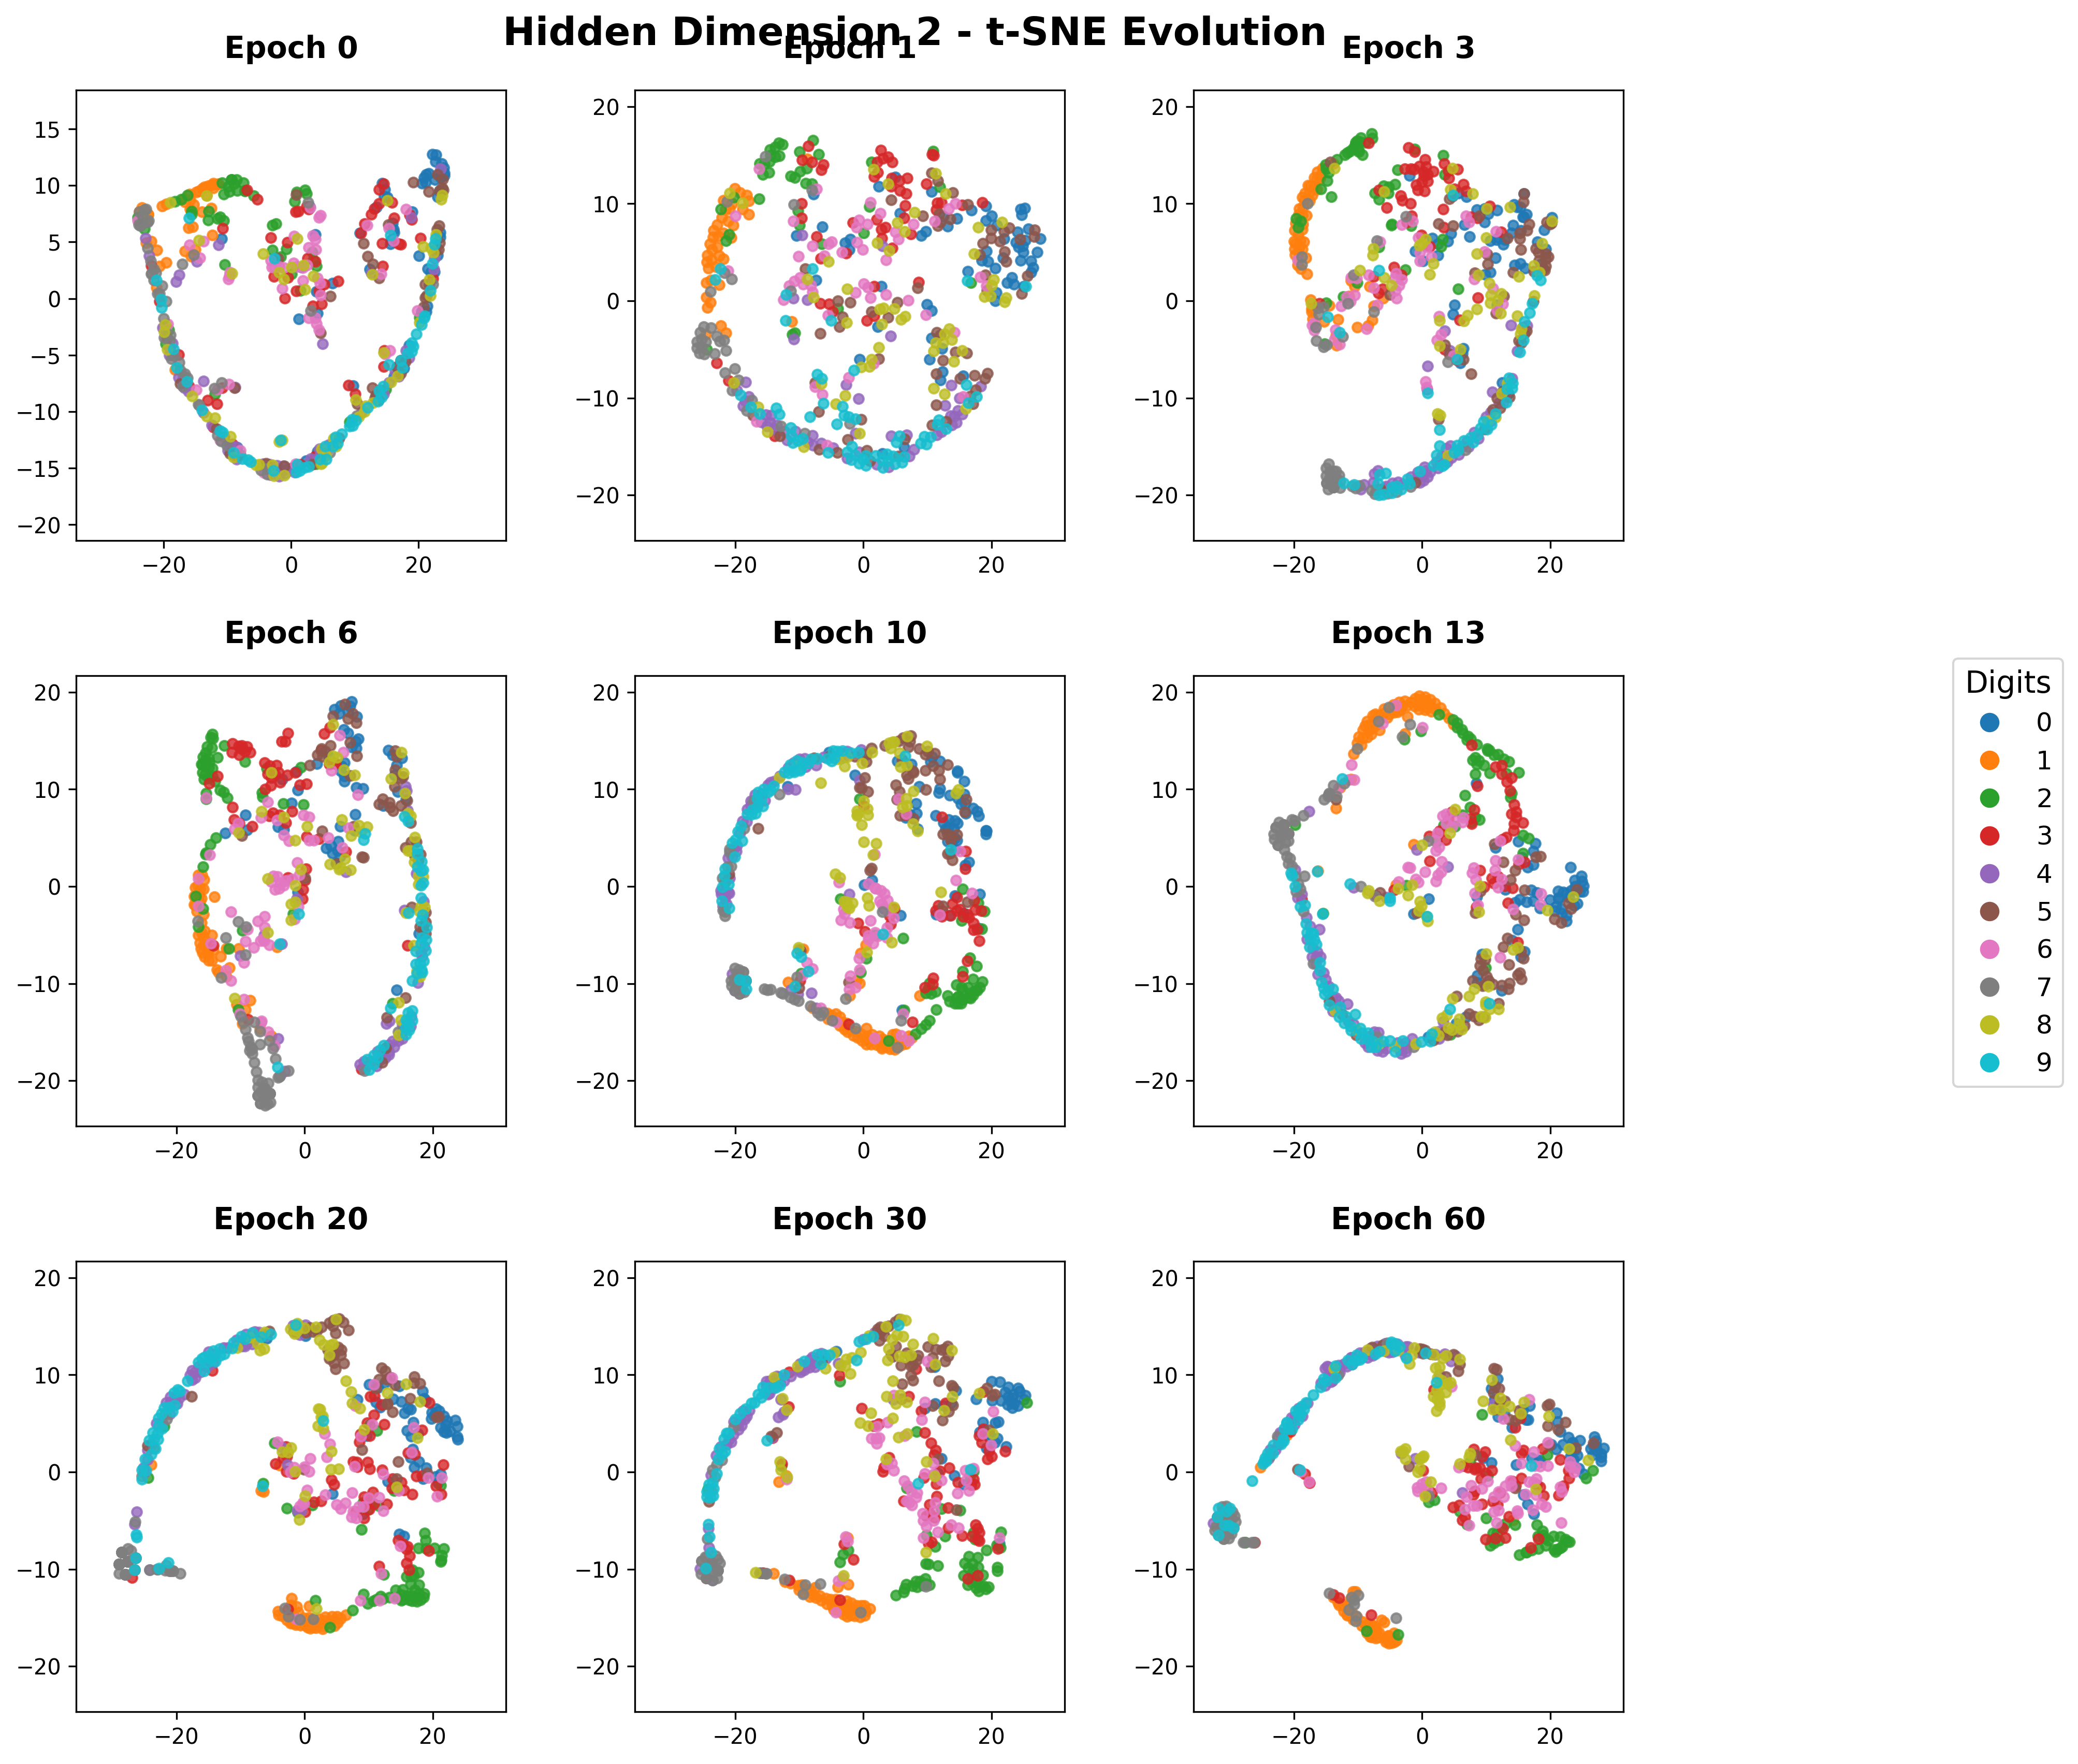
\includegraphics[width=0.8\textwidth]{../images/pa/tsne_evolution_hidden_2.png}
    \caption{隐层神经元数为2时的t-SNE可视化演化}
    \label{fig:2}
\end{figure}
\begin{figure}[H]
    \centering
    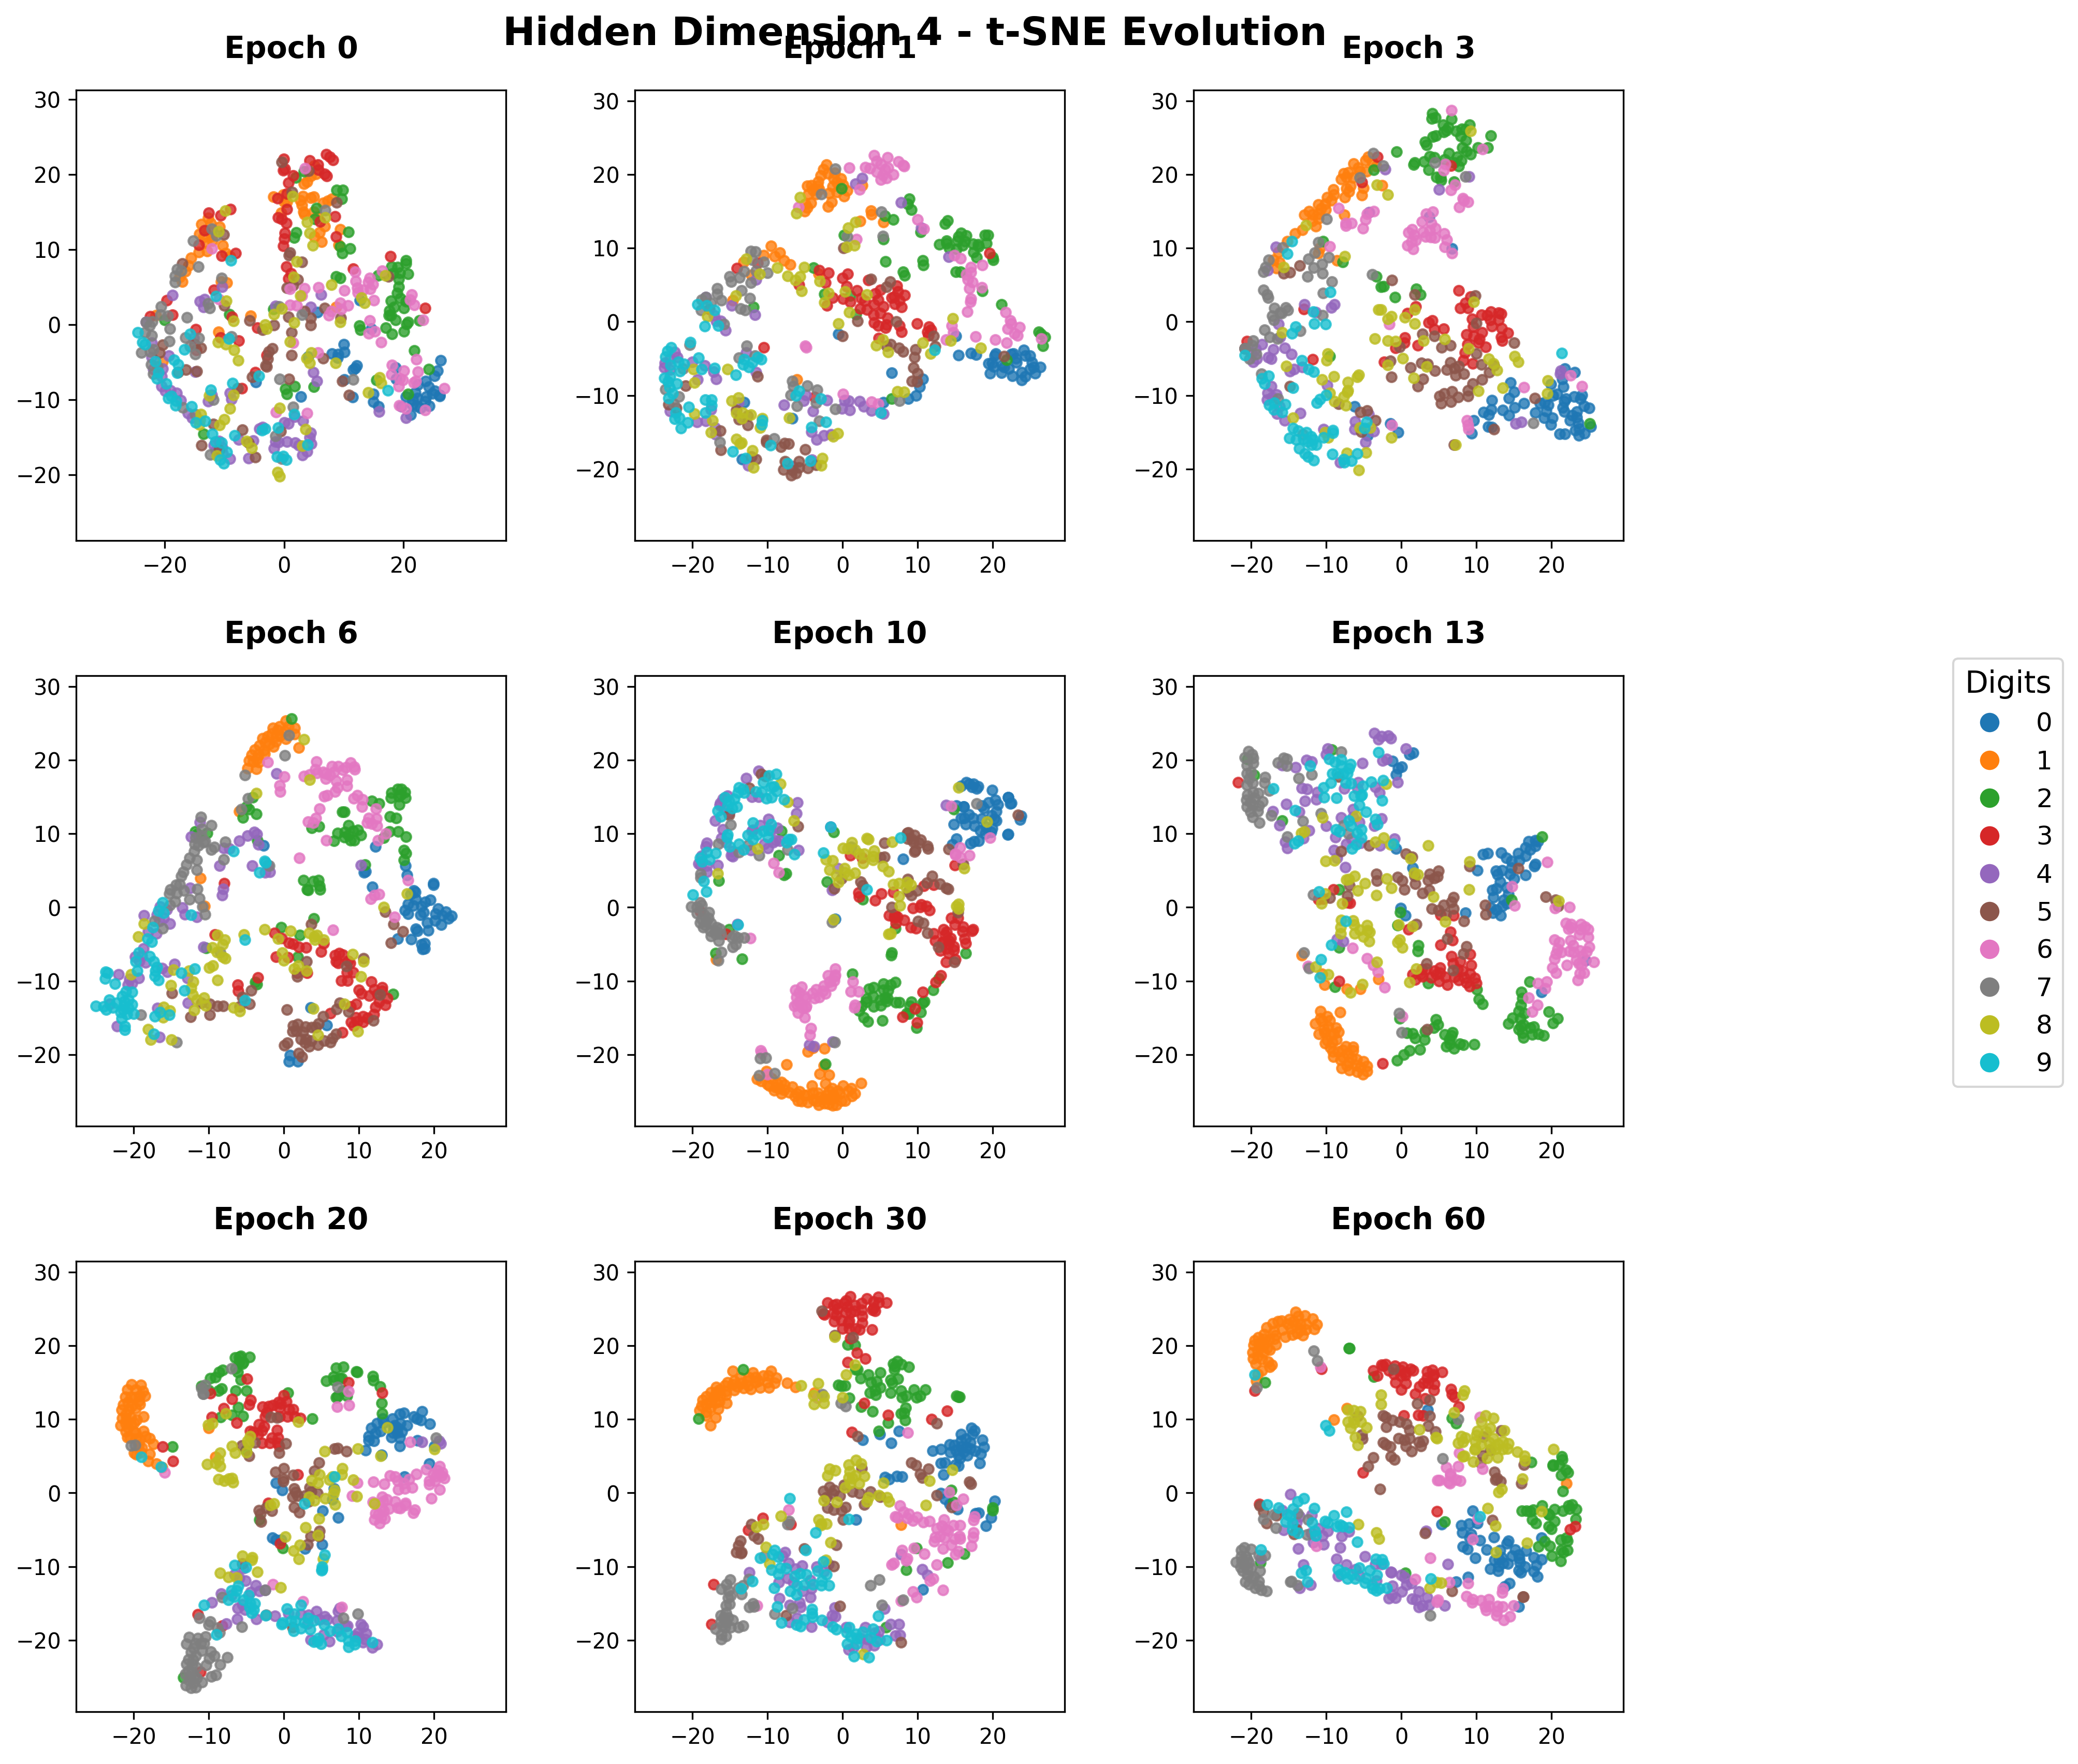
\includegraphics[width=0.8\textwidth]{../images/pa/tsne_evolution_hidden_4.png}
    \caption{隐层神经元数为4时的t-SNE可视化演化}
    \label{fig:4}
\end{figure}
\begin{figure}[H]
    \centering
    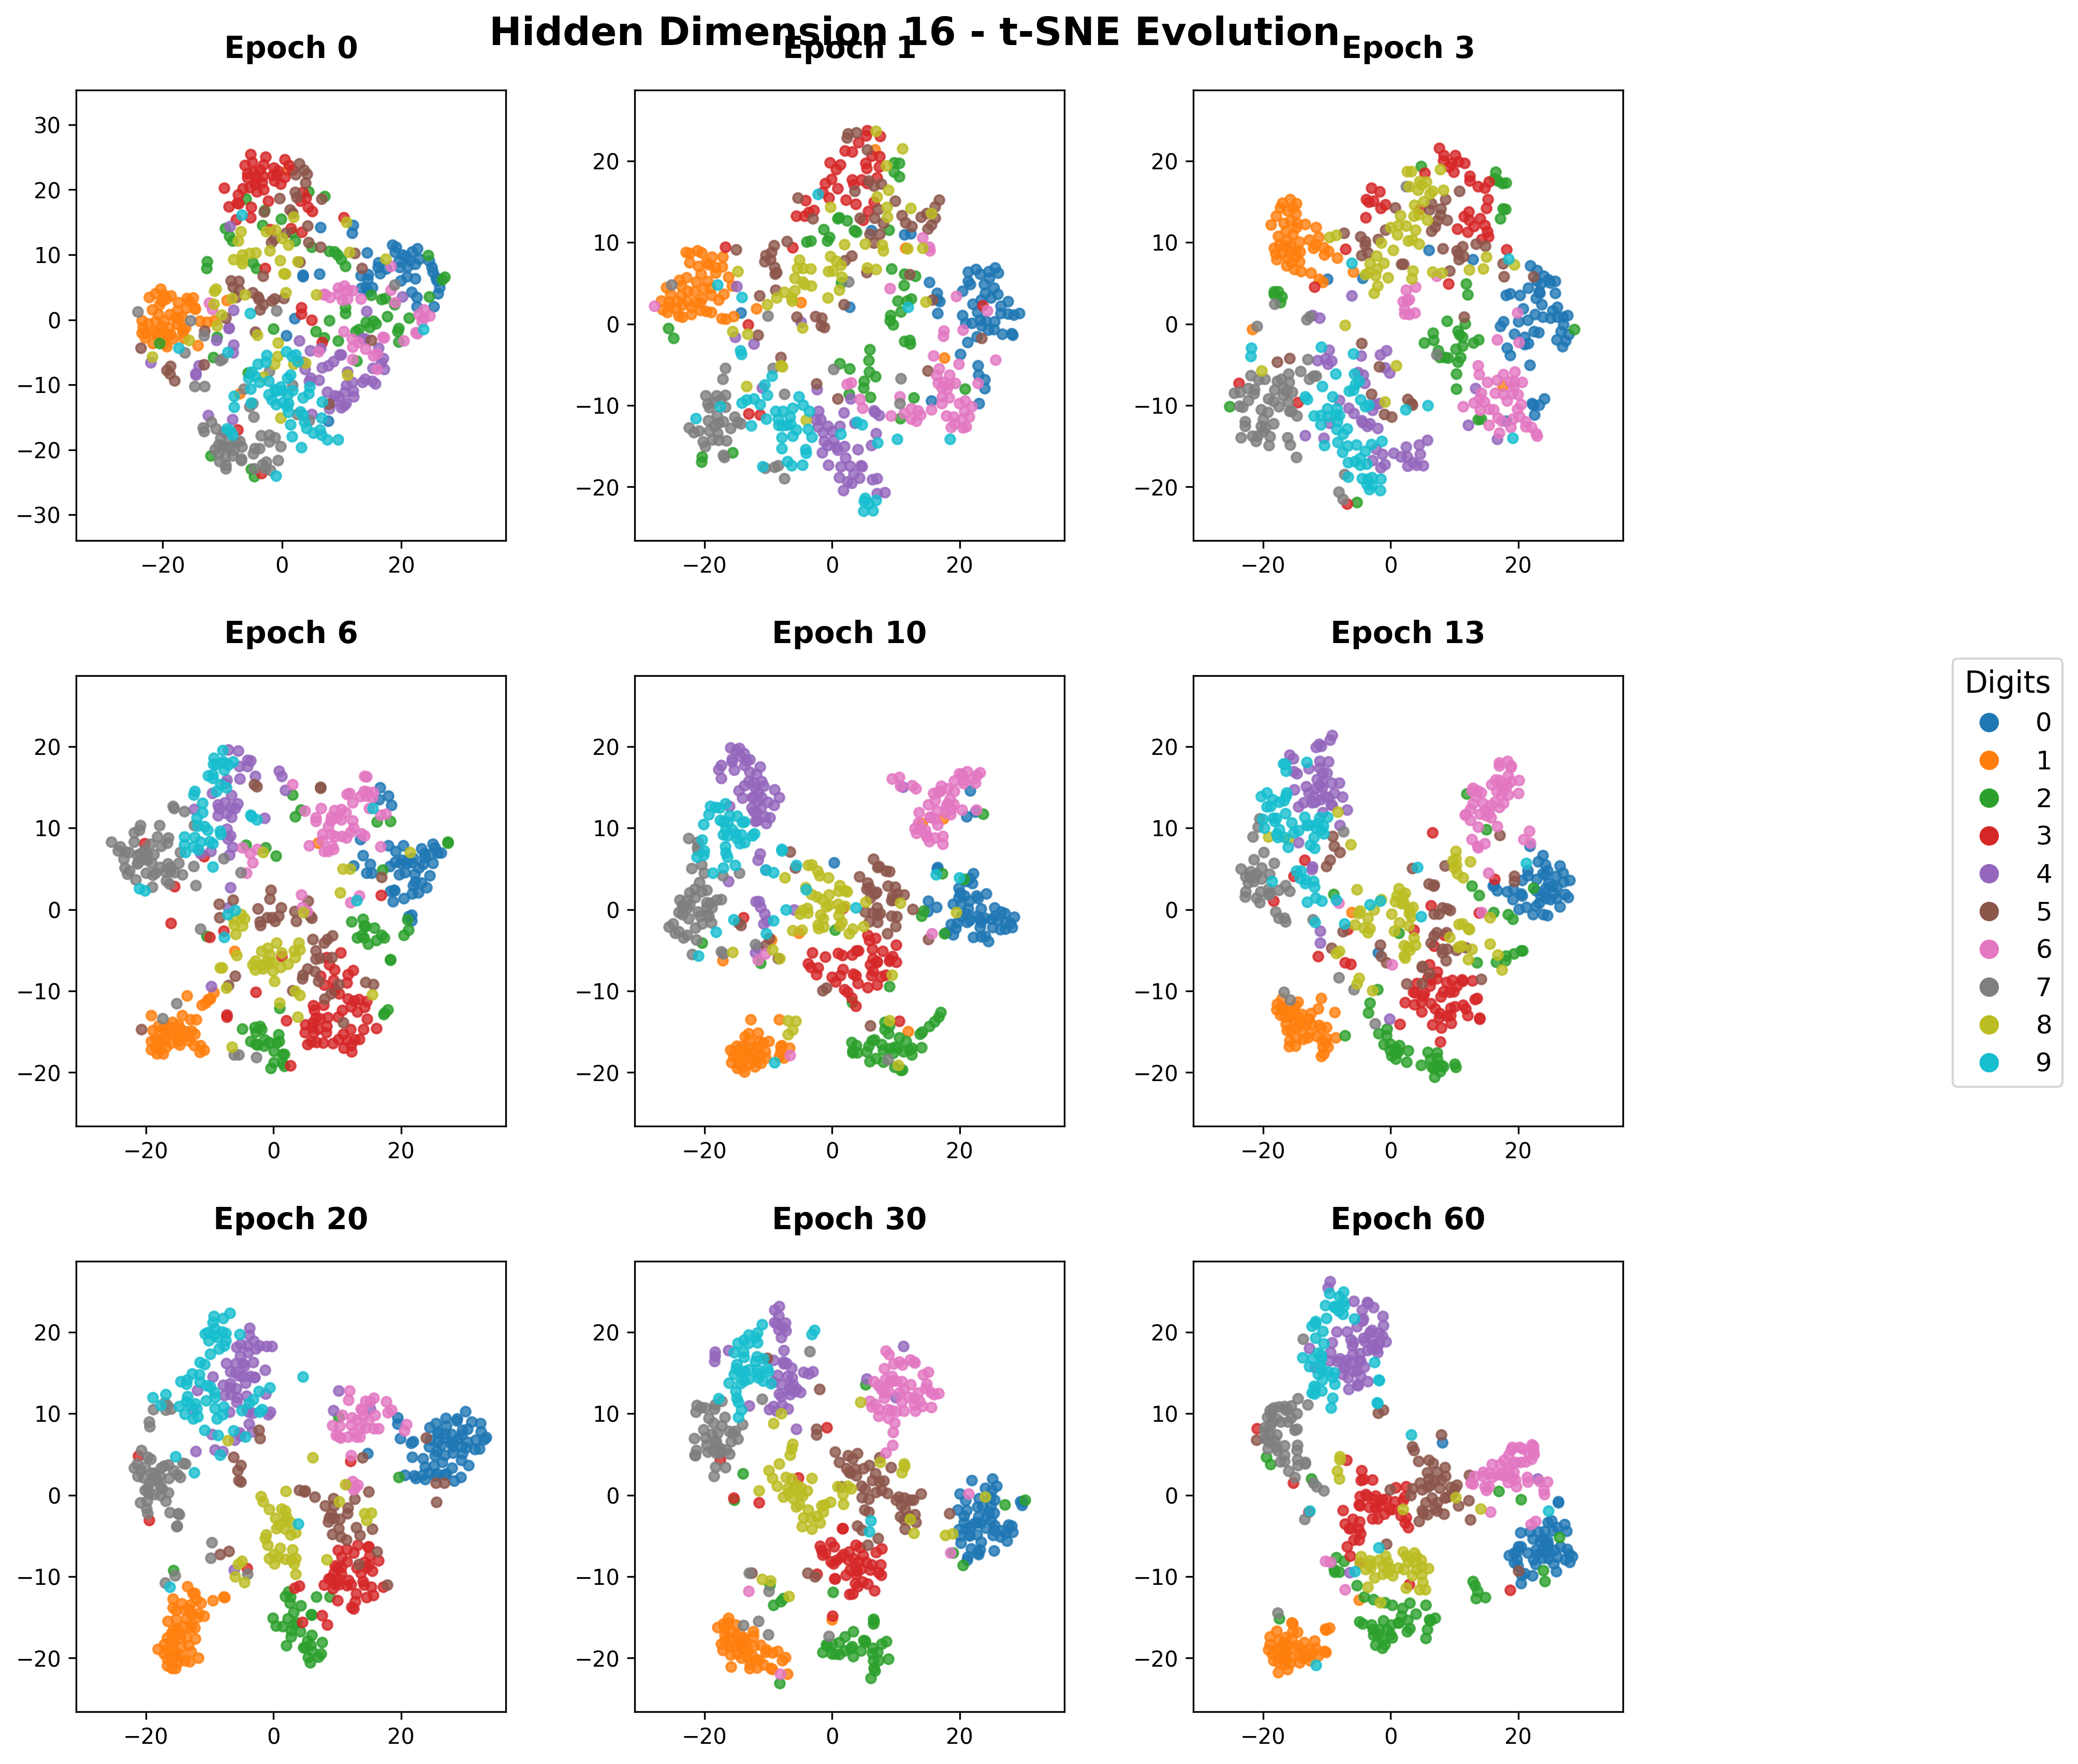
\includegraphics[width=0.8\textwidth]{../images/pa/tsne_evolution_hidden_16.png}
    \caption{隐层神经元数为16时的t-SNE可视化演化}
    \label{fig:16}
\end{figure}
\begin{figure}[H]
    \centering
    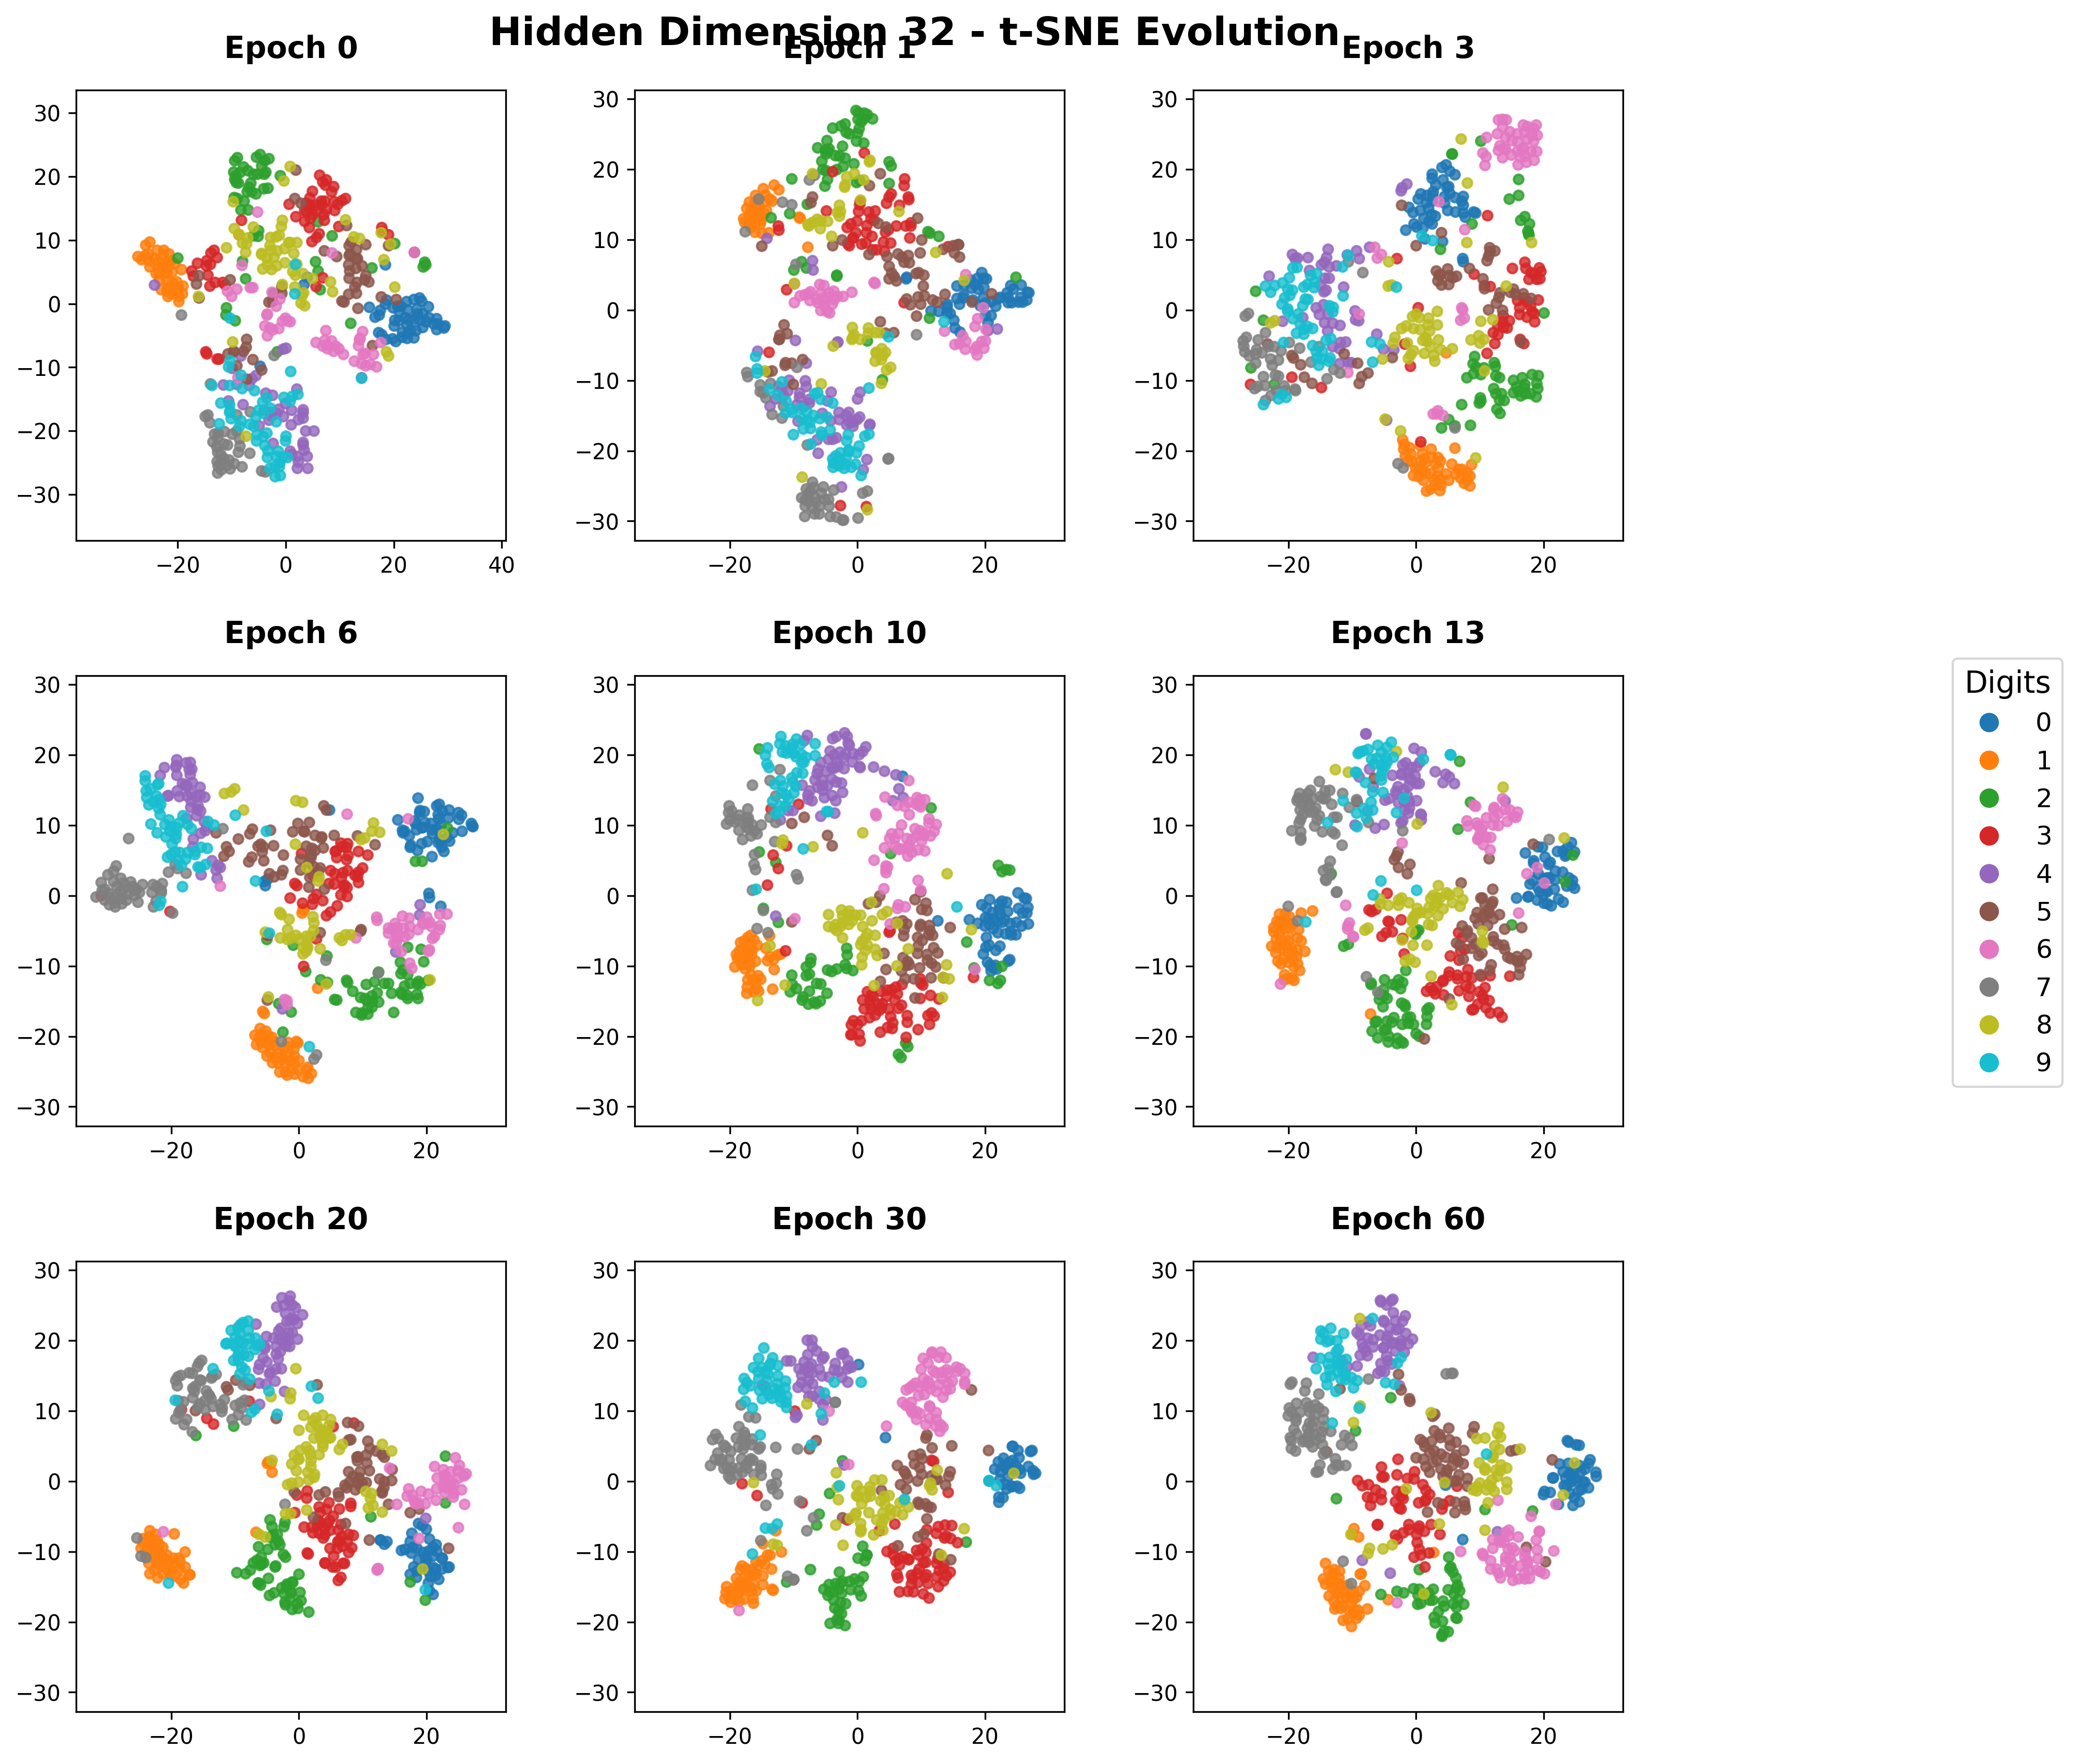
\includegraphics[width=0.8\textwidth]{../images/pa/tsne_evolution_hidden_32.png}
    \caption{隐层神经元数为32时的t-SNE可视化演化}
    \label{fig:32}
\end{figure}
\begin{figure}[H]
    \centering
    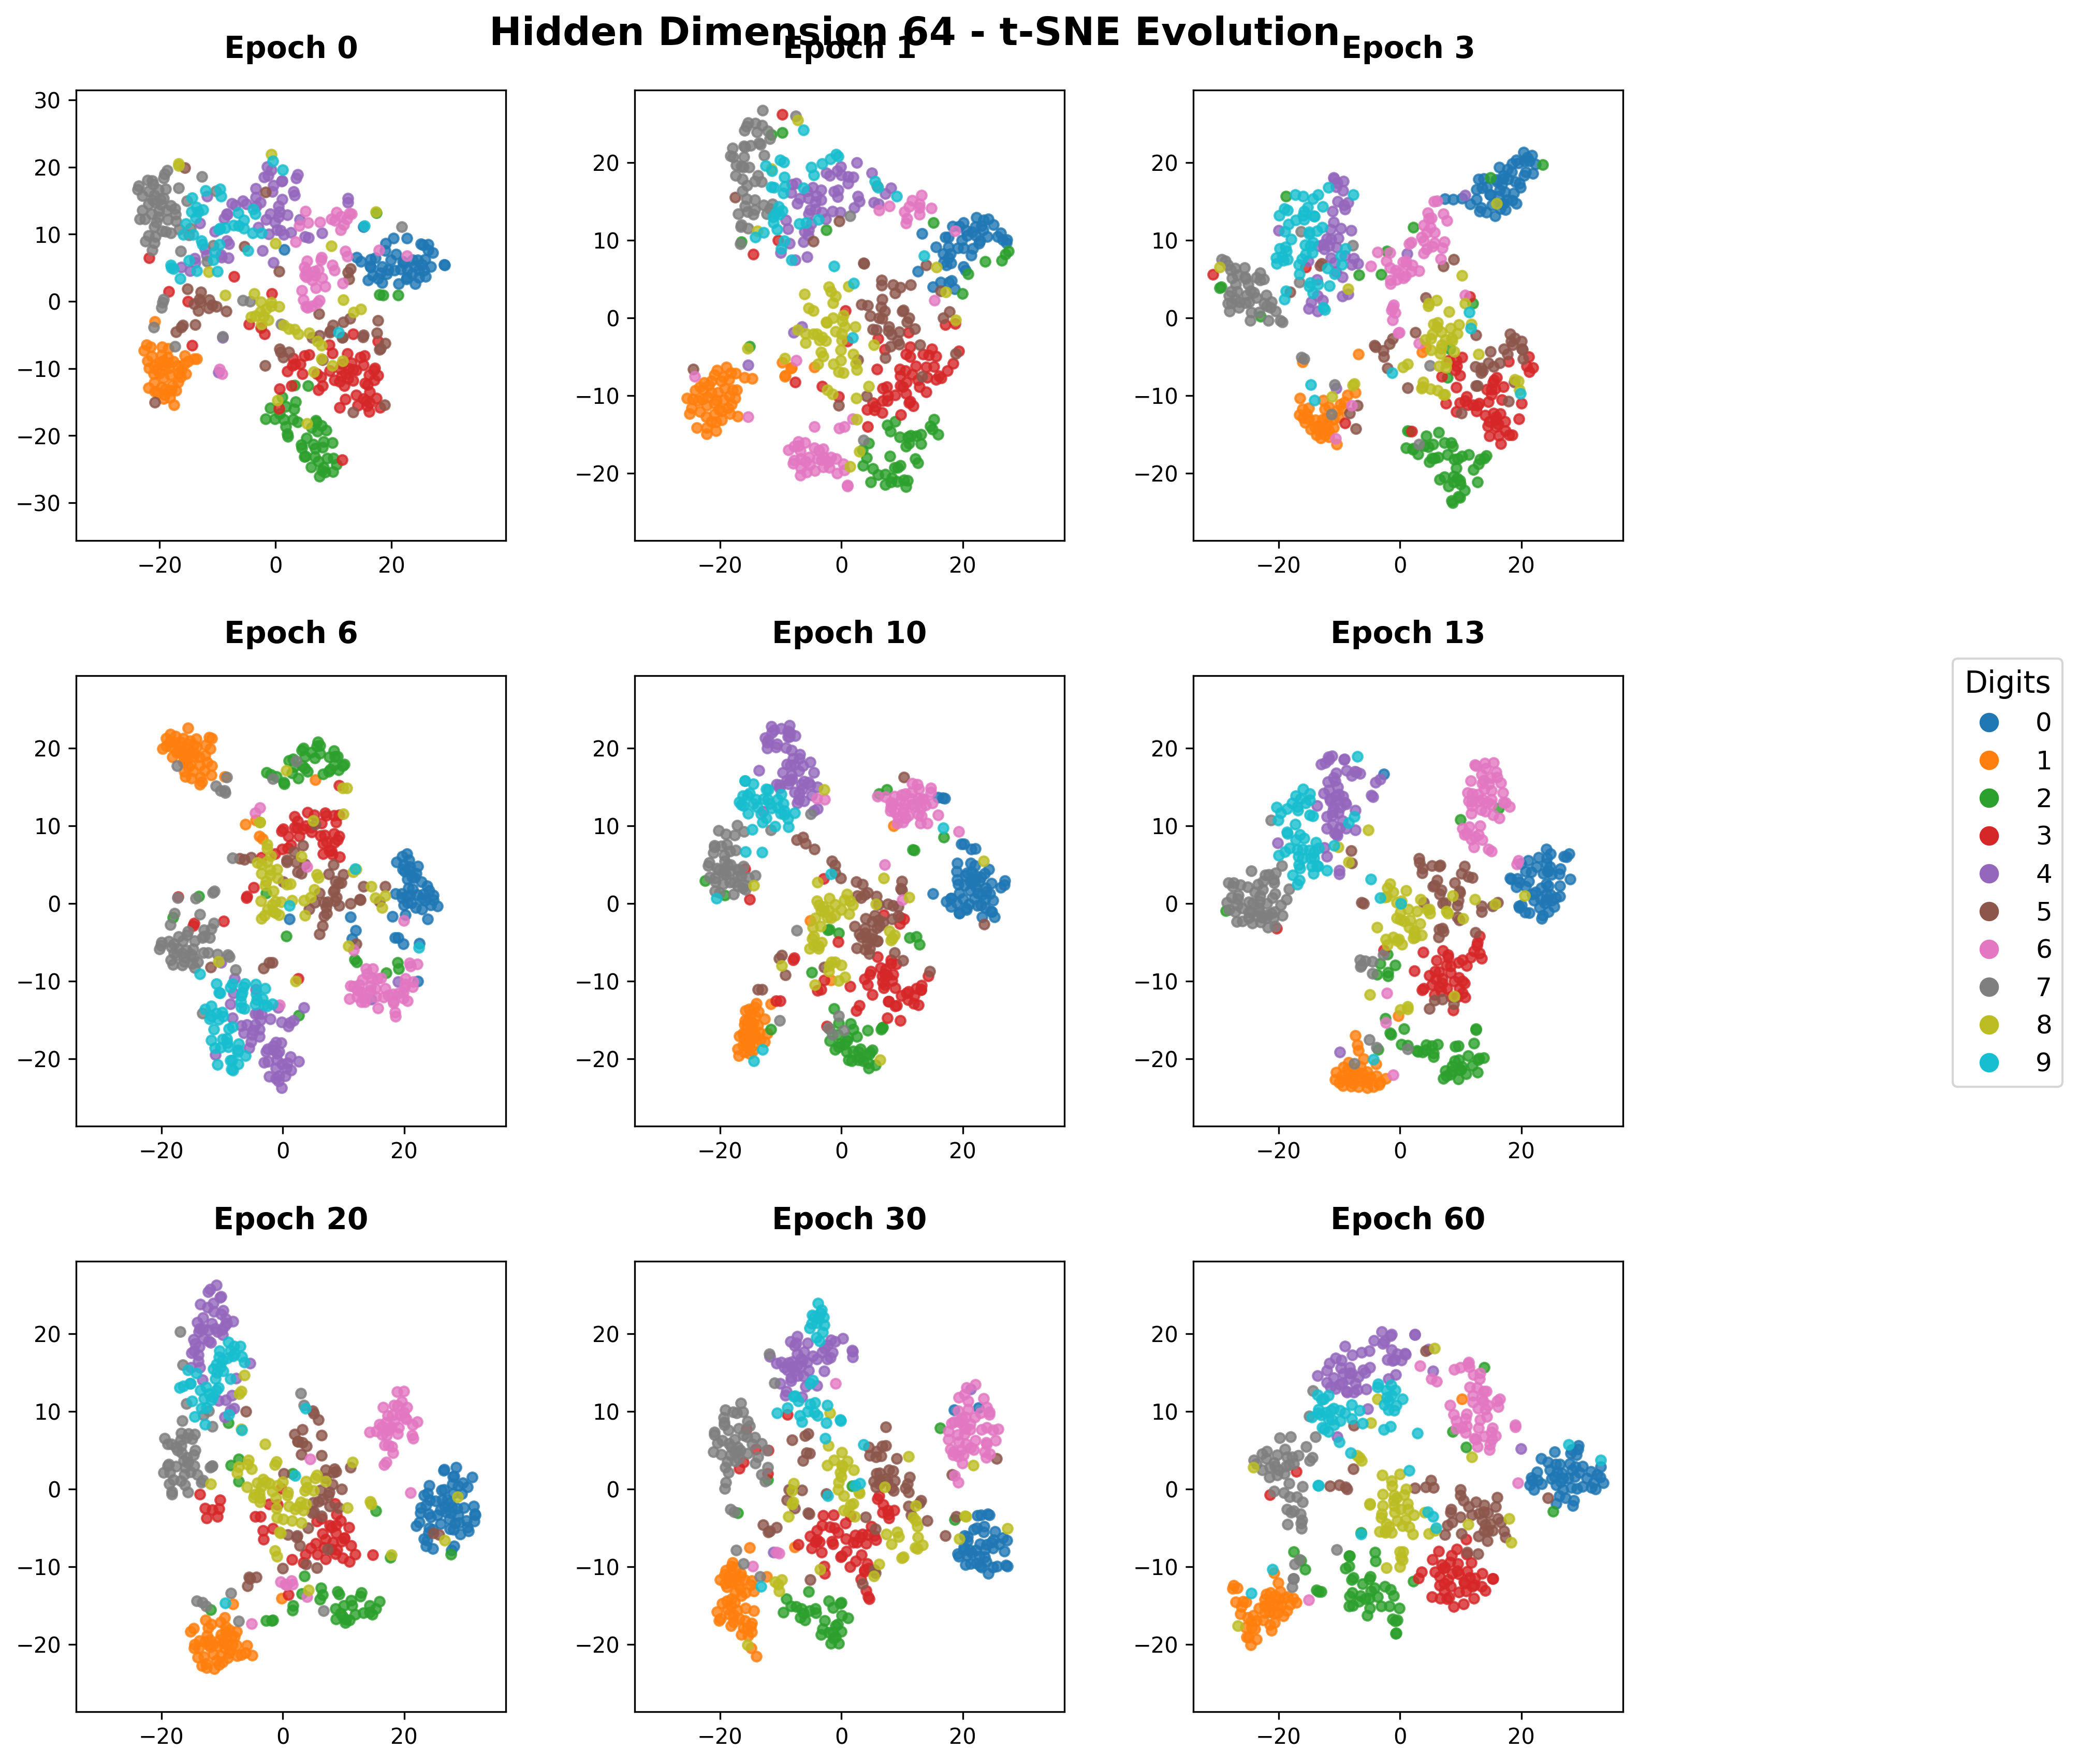
\includegraphics[width=0.8\textwidth]{../images/pa/tsne_evolution_hidden_64.png}
    \caption{隐层神经元数为64时的t-SNE可视化演化}
    \label{fig:64}
\end{figure}
\begin{figure}[H]
    \centering
    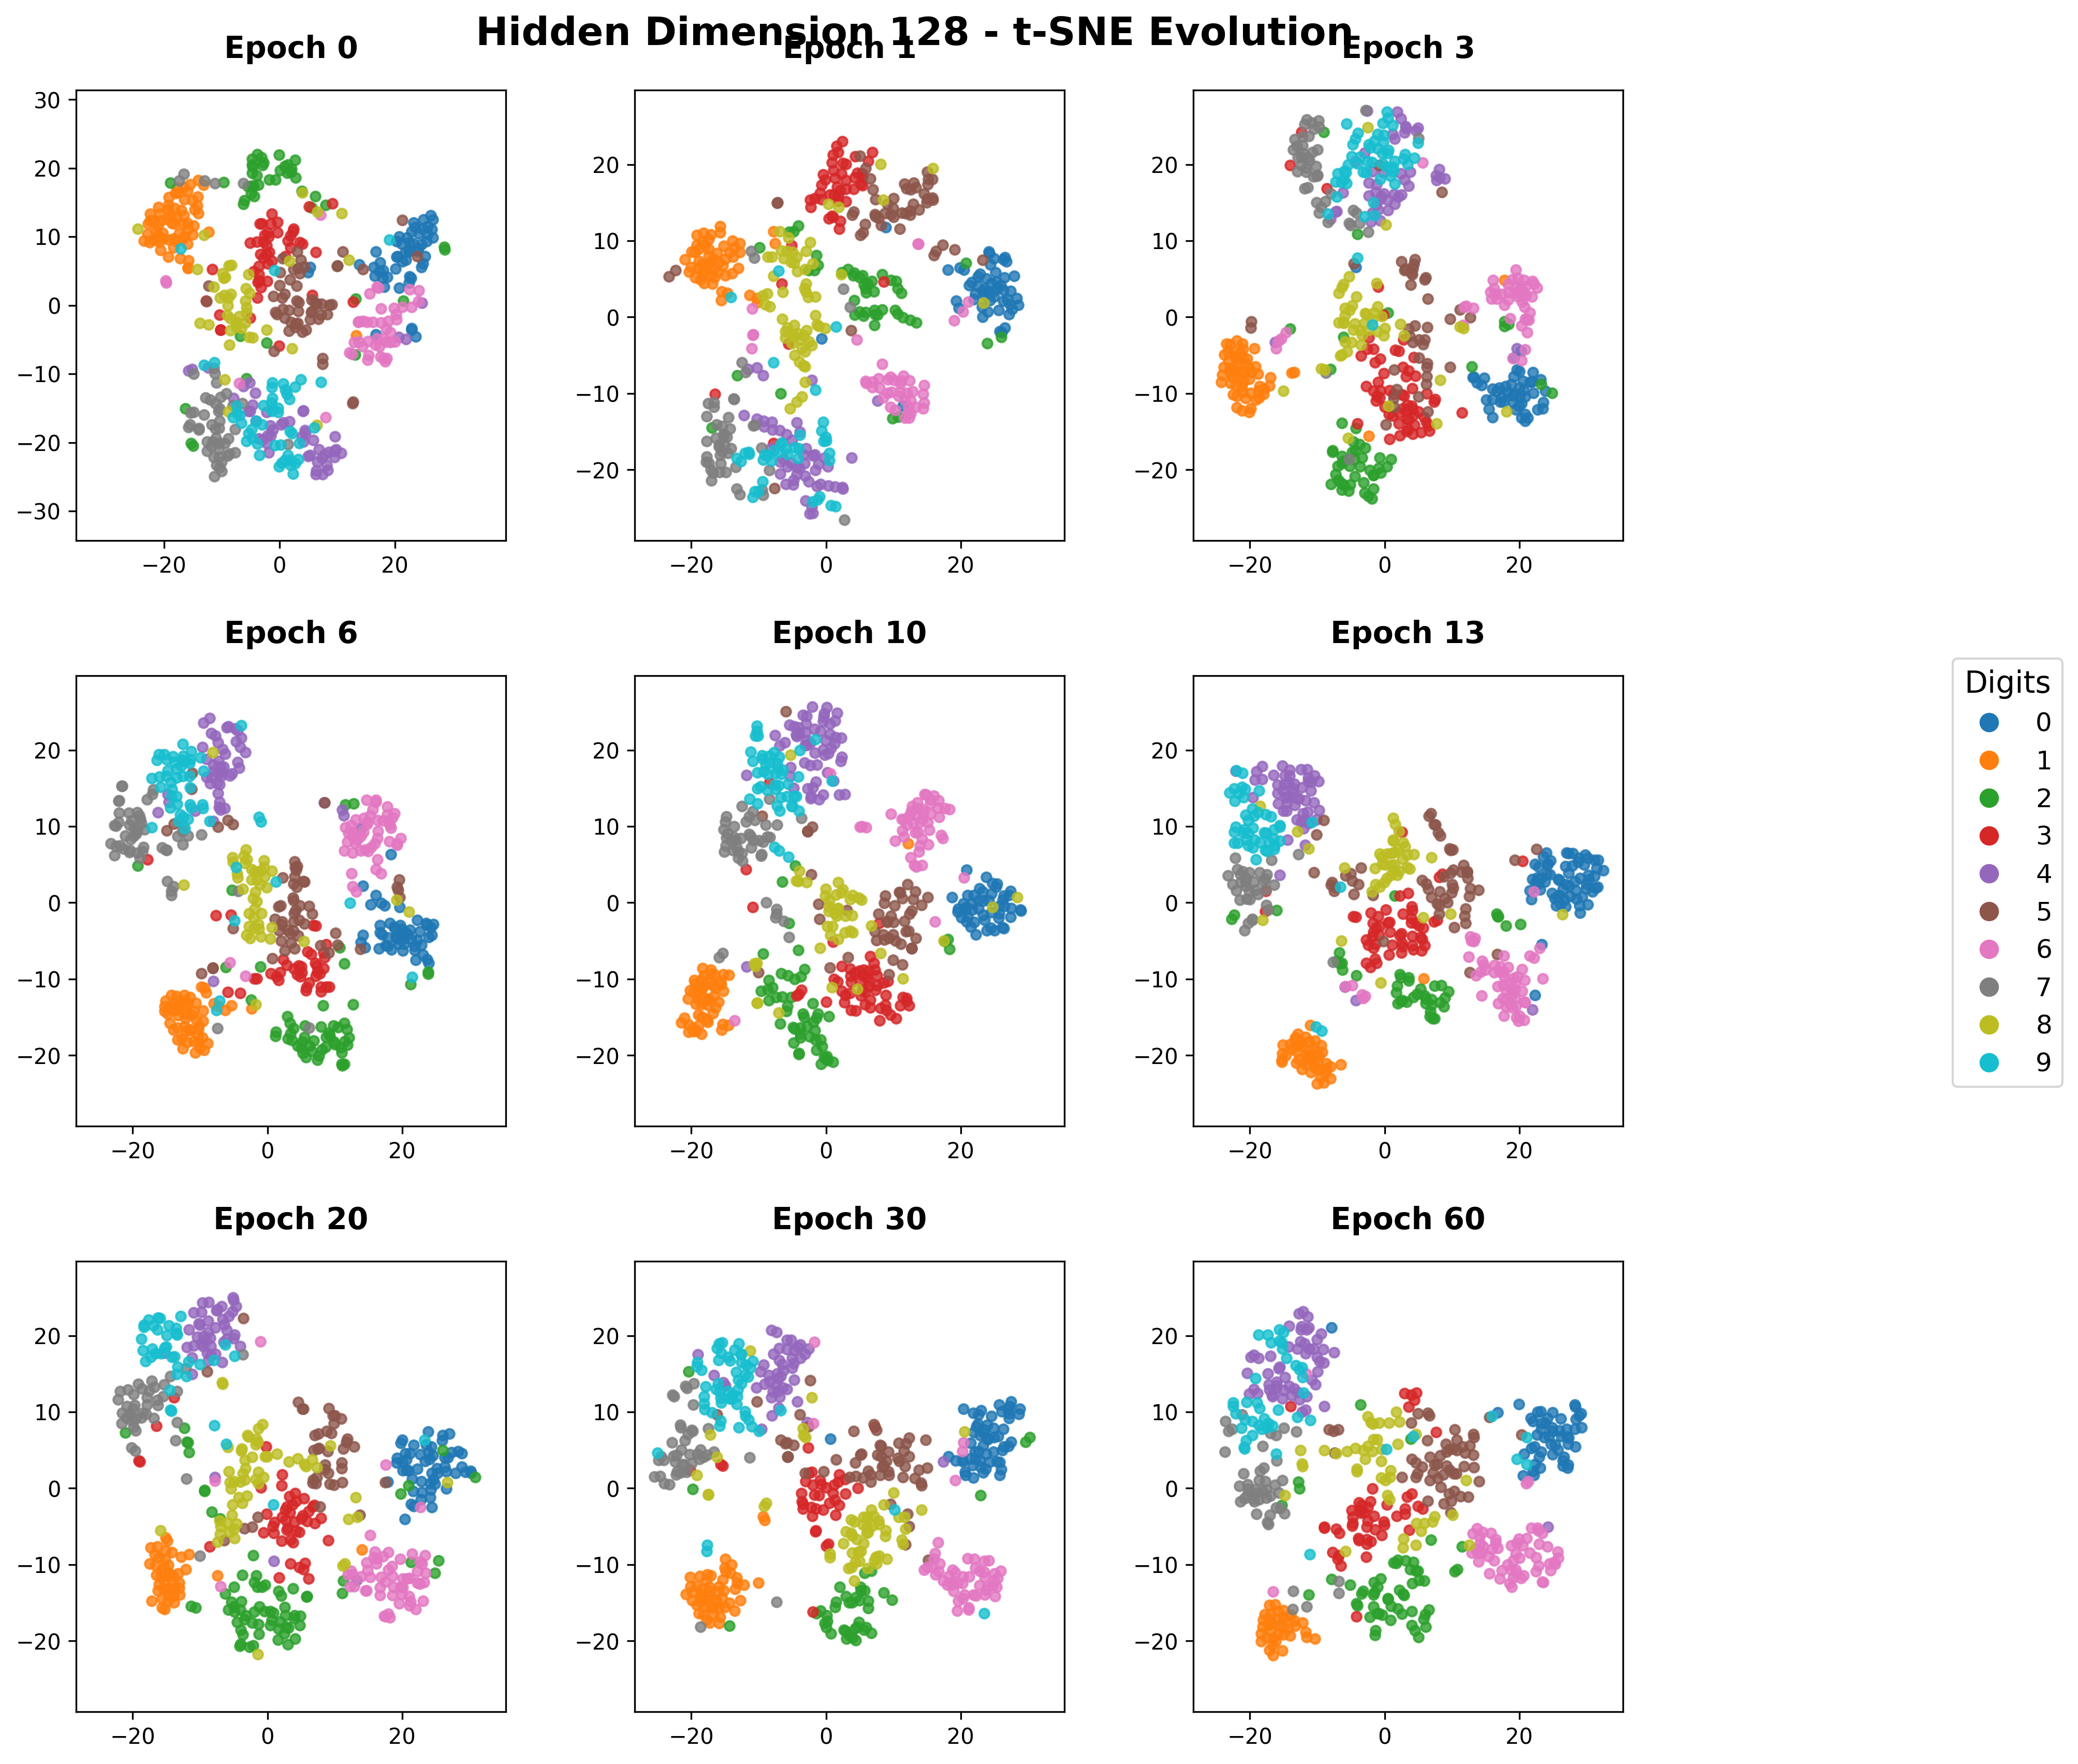
\includegraphics[width=0.8\textwidth]{../images/pa/tsne_evolution_hidden_128.png}
    \caption{隐层神经元数为128时的t-SNE可视化演化}
    \label{fig:128}
\end{figure}
\begin{figure}[H]
    \centering
    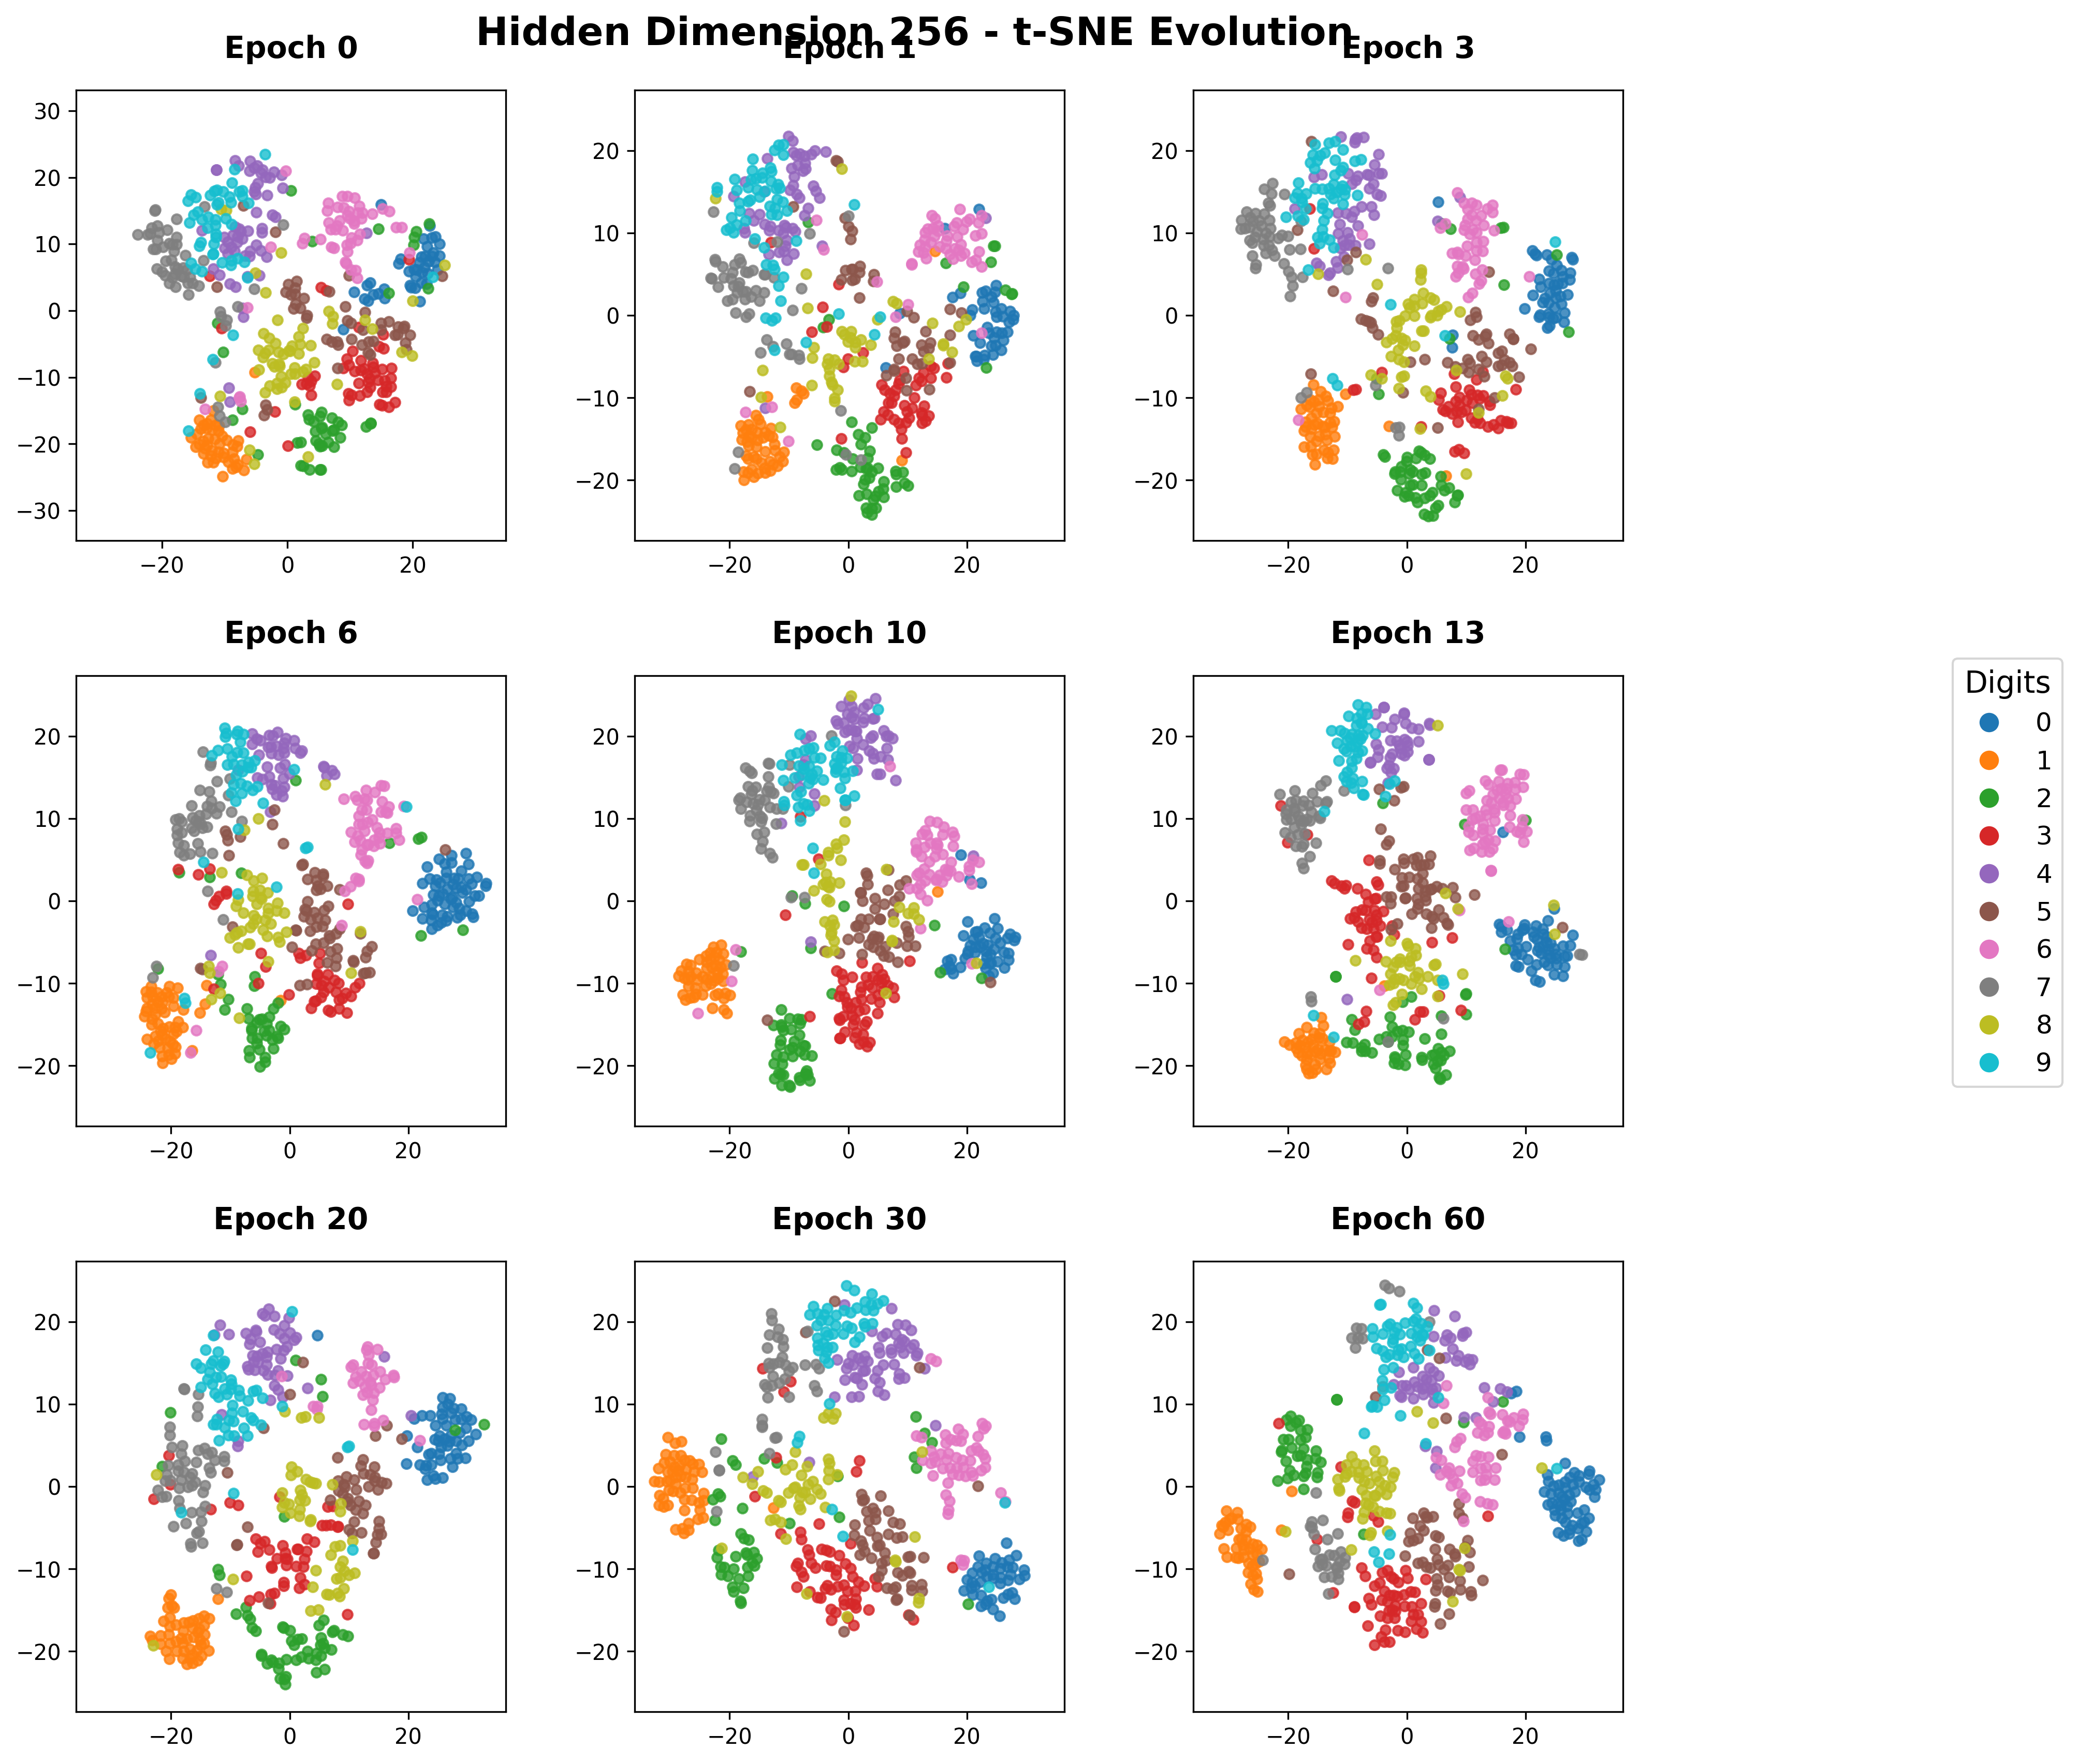
\includegraphics[width=0.8\textwidth]{../images/pa/tsne_evolution_hidden_256.png}
    \caption{隐层神经元数为256时的t-SNE可视化演化}
    \label{fig:256}
\end{figure}
\begin{figure}[H]
    \centering
    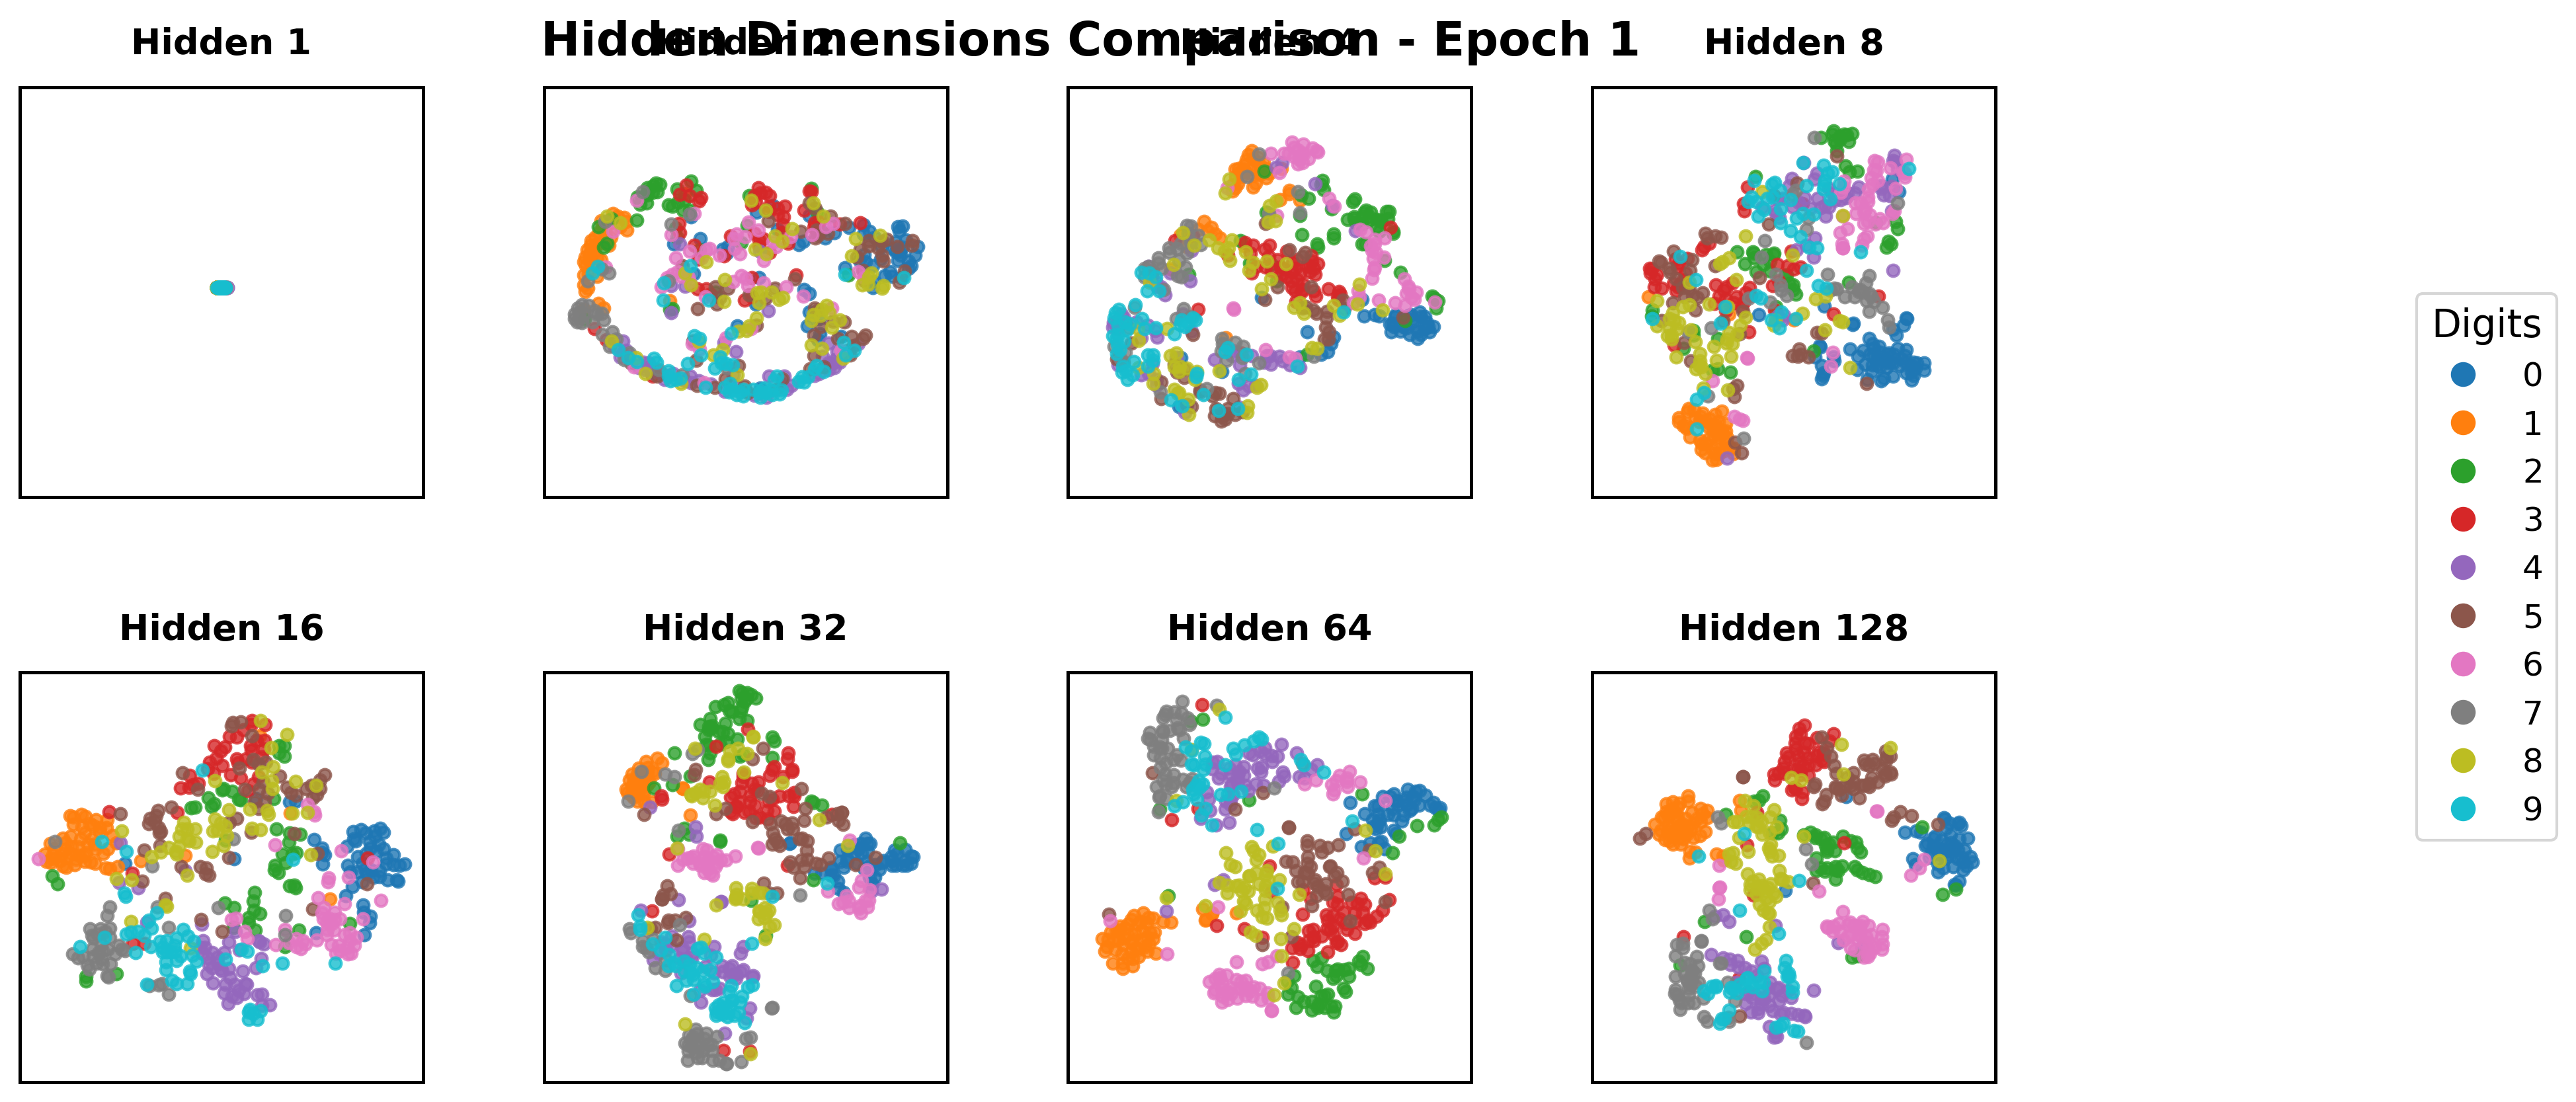
\includegraphics[width=0.8\textwidth]{../images/pa/tsne_comparison_epoch_1.png}
    \caption{t-SNE可视化对比(epoch=1)}
    \label{fig:11}
\end{figure}

\section{冻结实验结果}\label{sec:feature_extractor_classifier}
\begin{figure}[H]
    \centering
    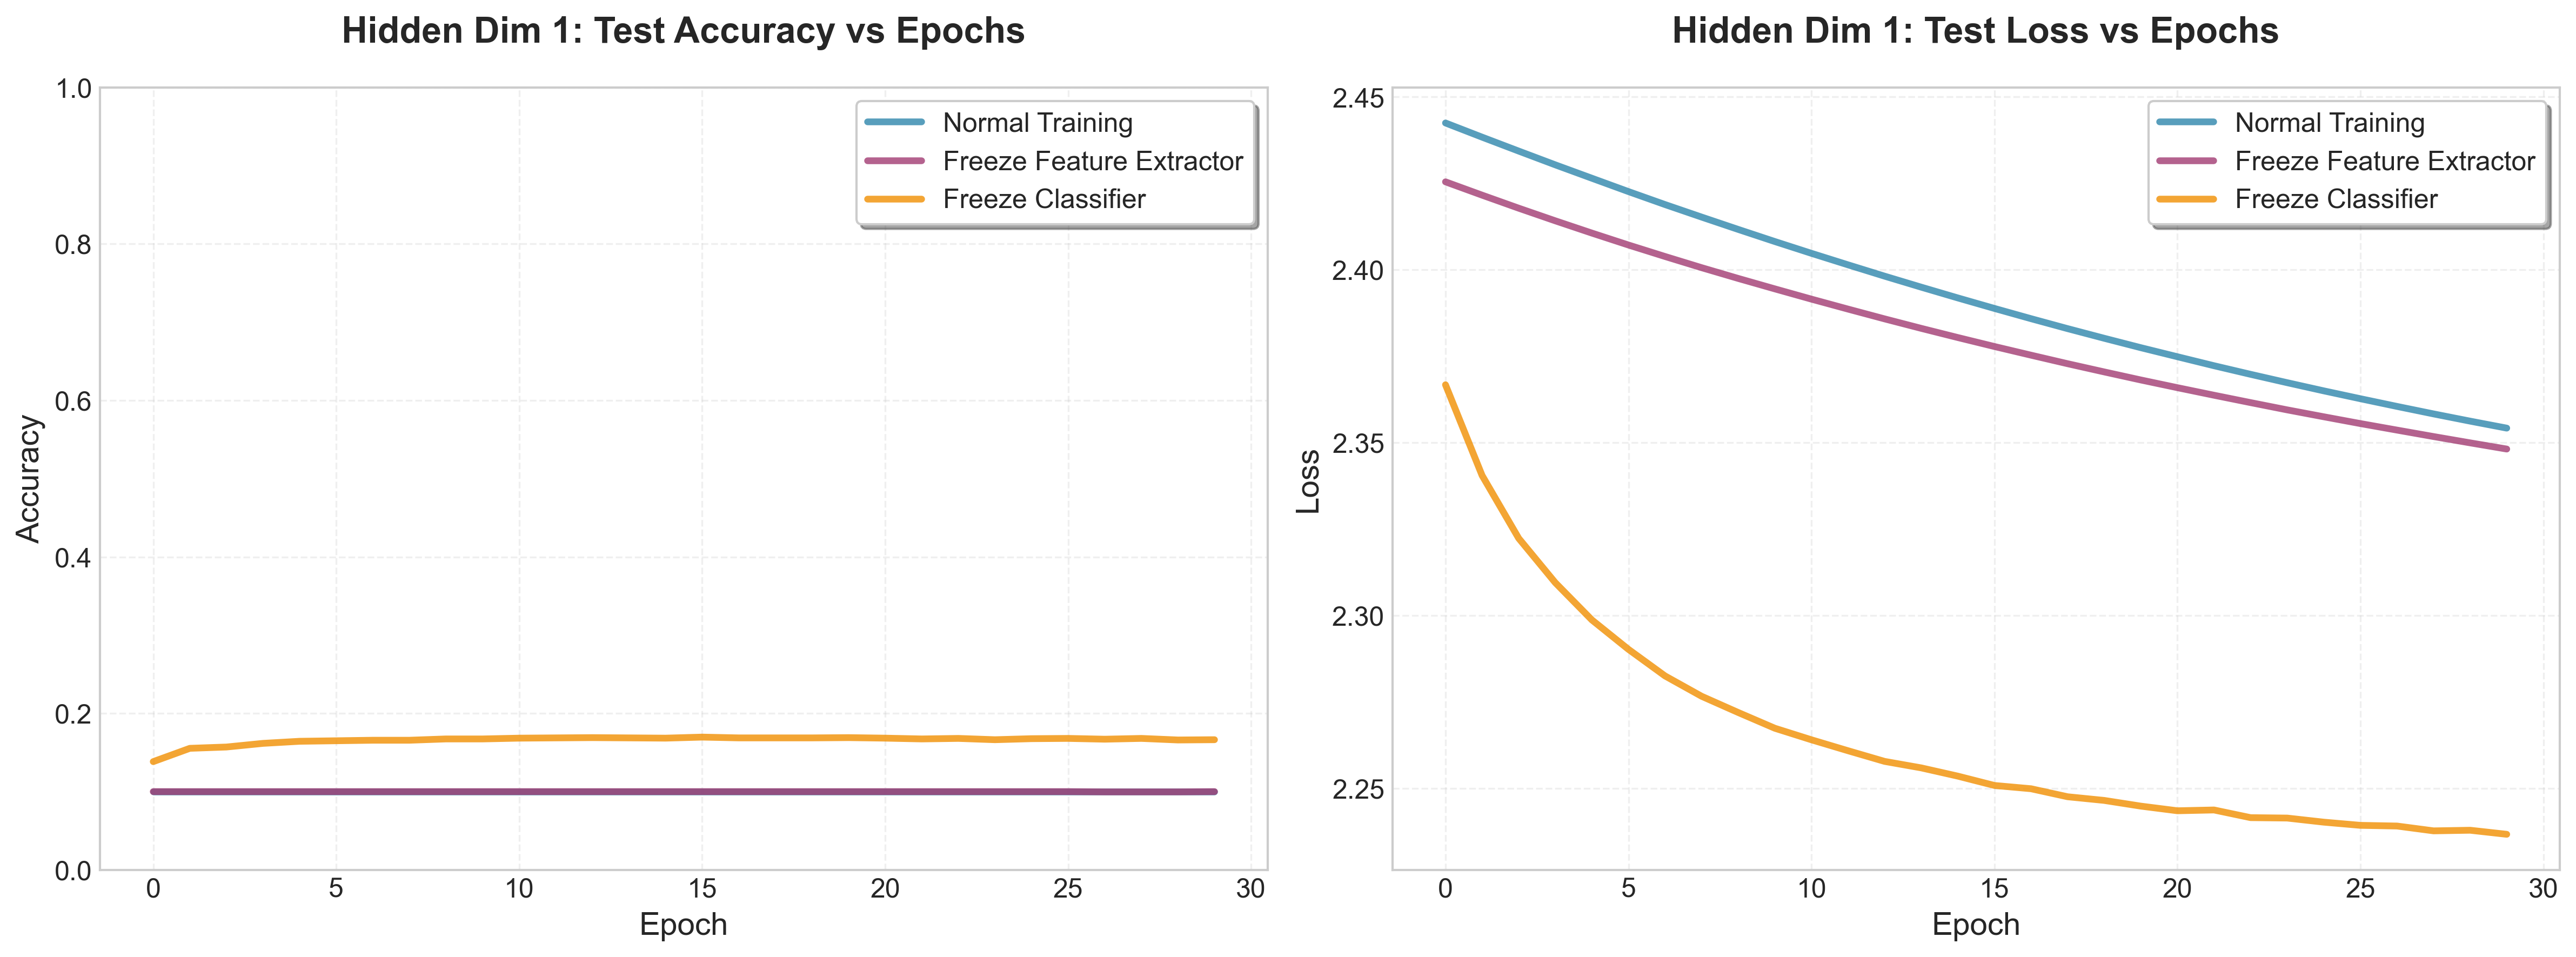
\includegraphics[width=0.8\textwidth]{../images/dd/hidden_1_comparison.png}
    \caption{冻结实验结果对比(隐藏层神经元数为1)}
    \label{fig:hidden_1_comparison.png}
\end{figure}
\begin{figure}[H]
    \centering
    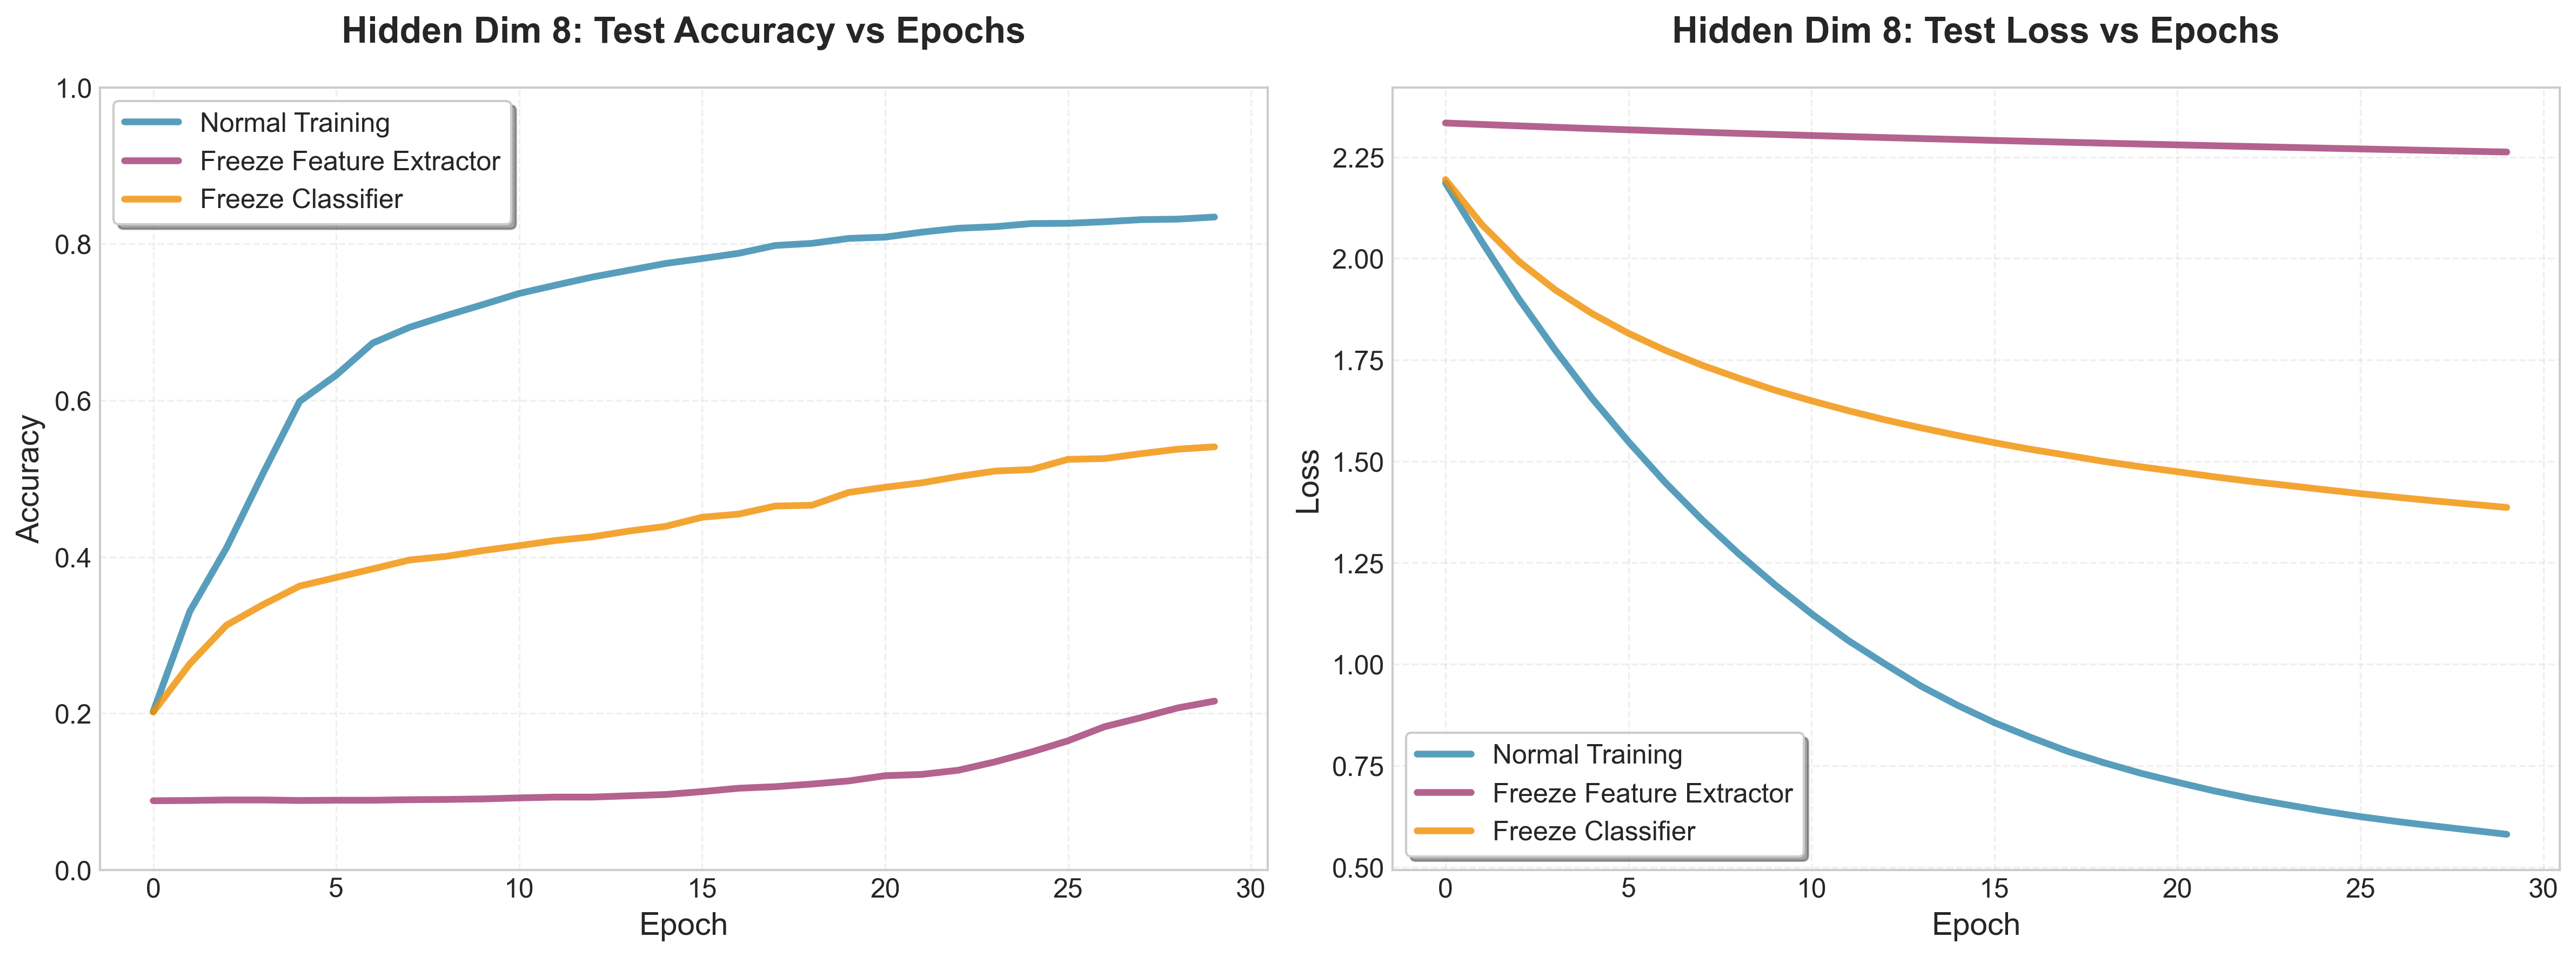
\includegraphics[width=0.8\textwidth]{../images/dd/hidden_8_comparison.png}
    \caption{冻结实验结果对比(隐藏层神经元数为8)}
    \label{fig:hidden_8_comparison.png}
\end{figure}
\begin{figure}[H]
    \centering
    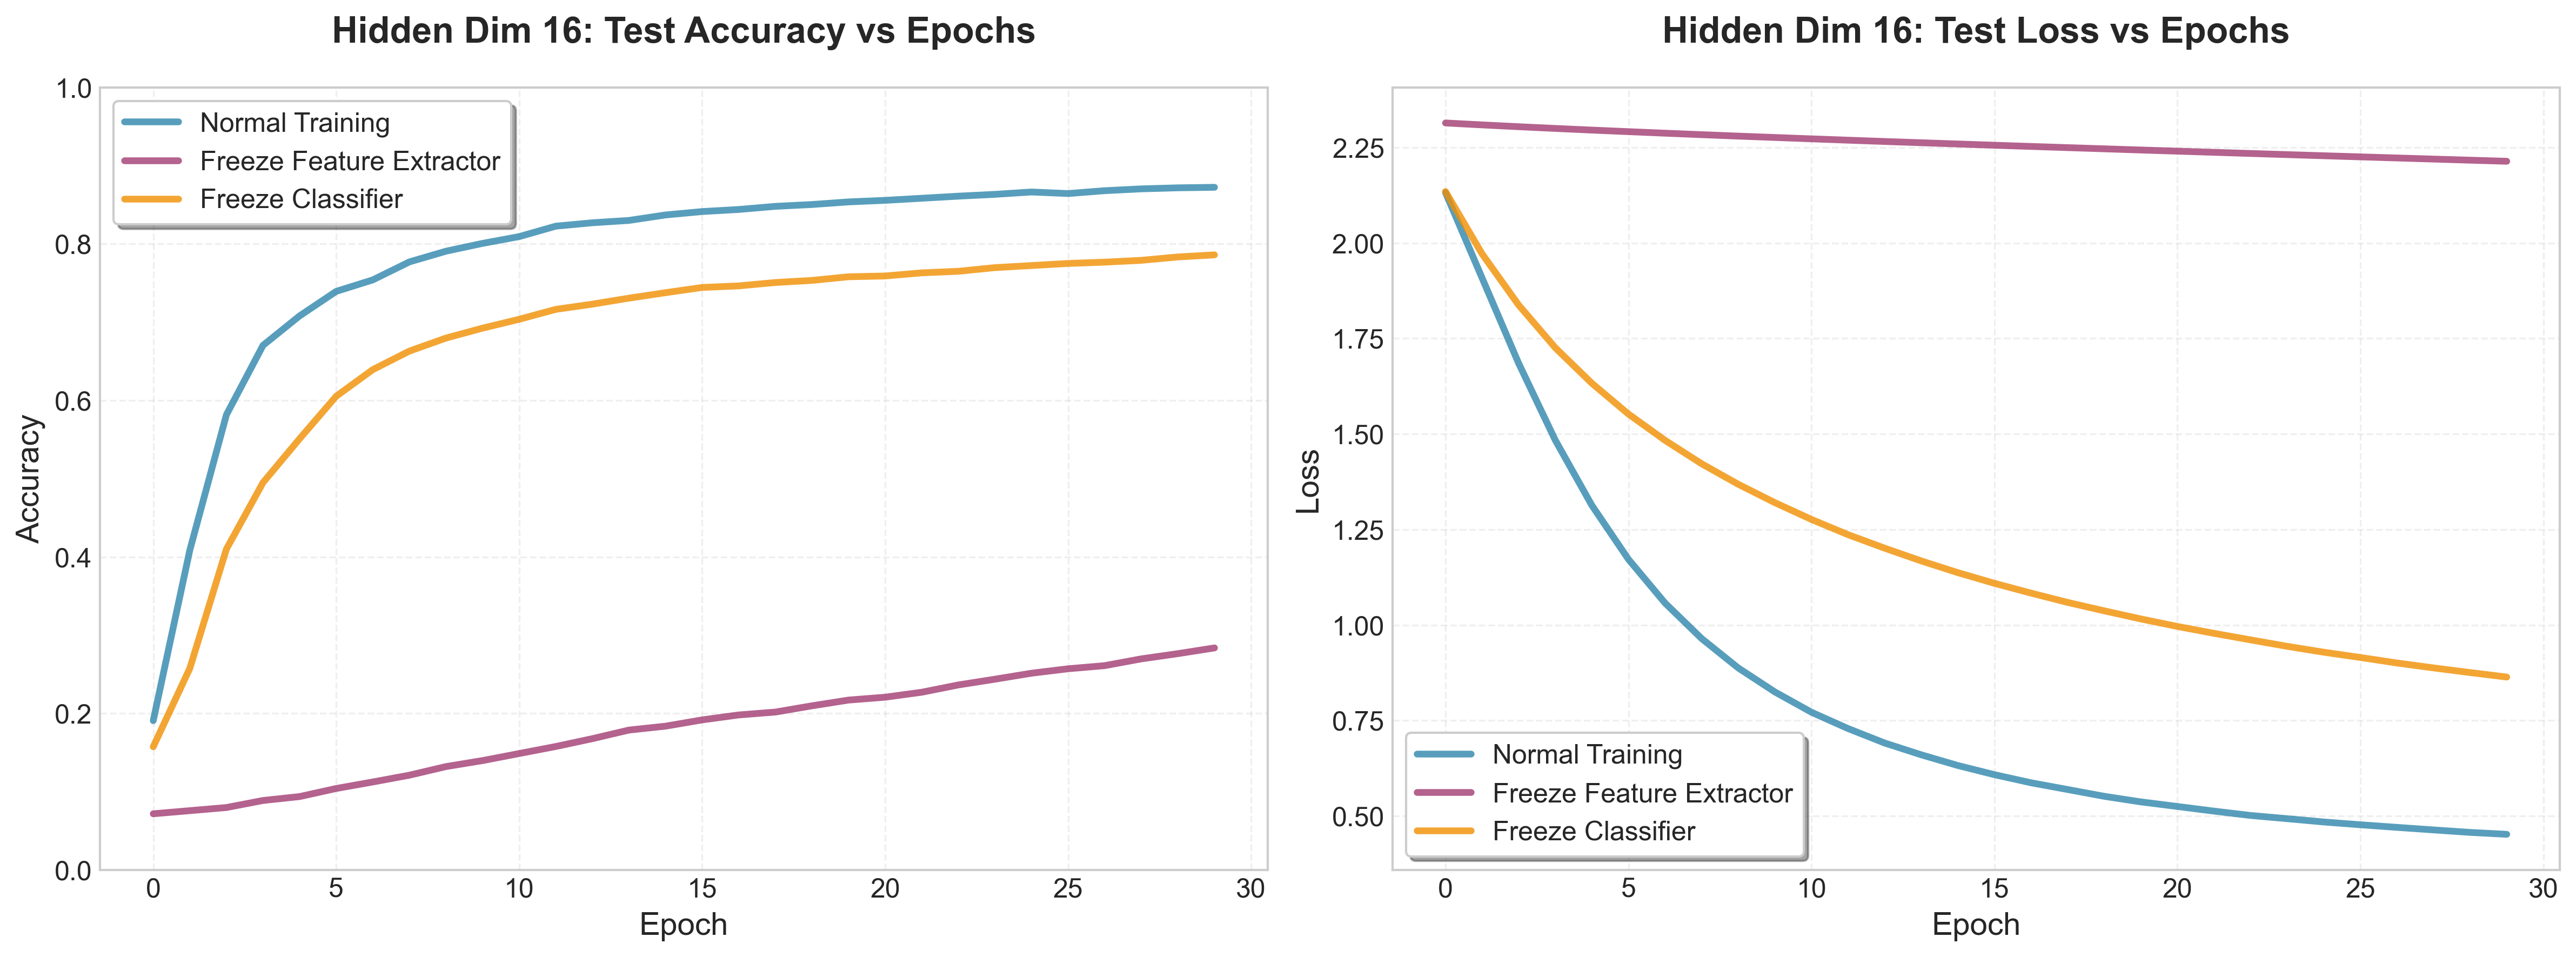
\includegraphics[width=0.8\textwidth]{../images/dd/hidden_16_comparison.png}
    \caption{冻结实验结果对比(隐藏层神经元数为16)}
    \label{fig:hidden_16_comparison.png}
\end{figure}
\begin{figure}[H]
    \centering
    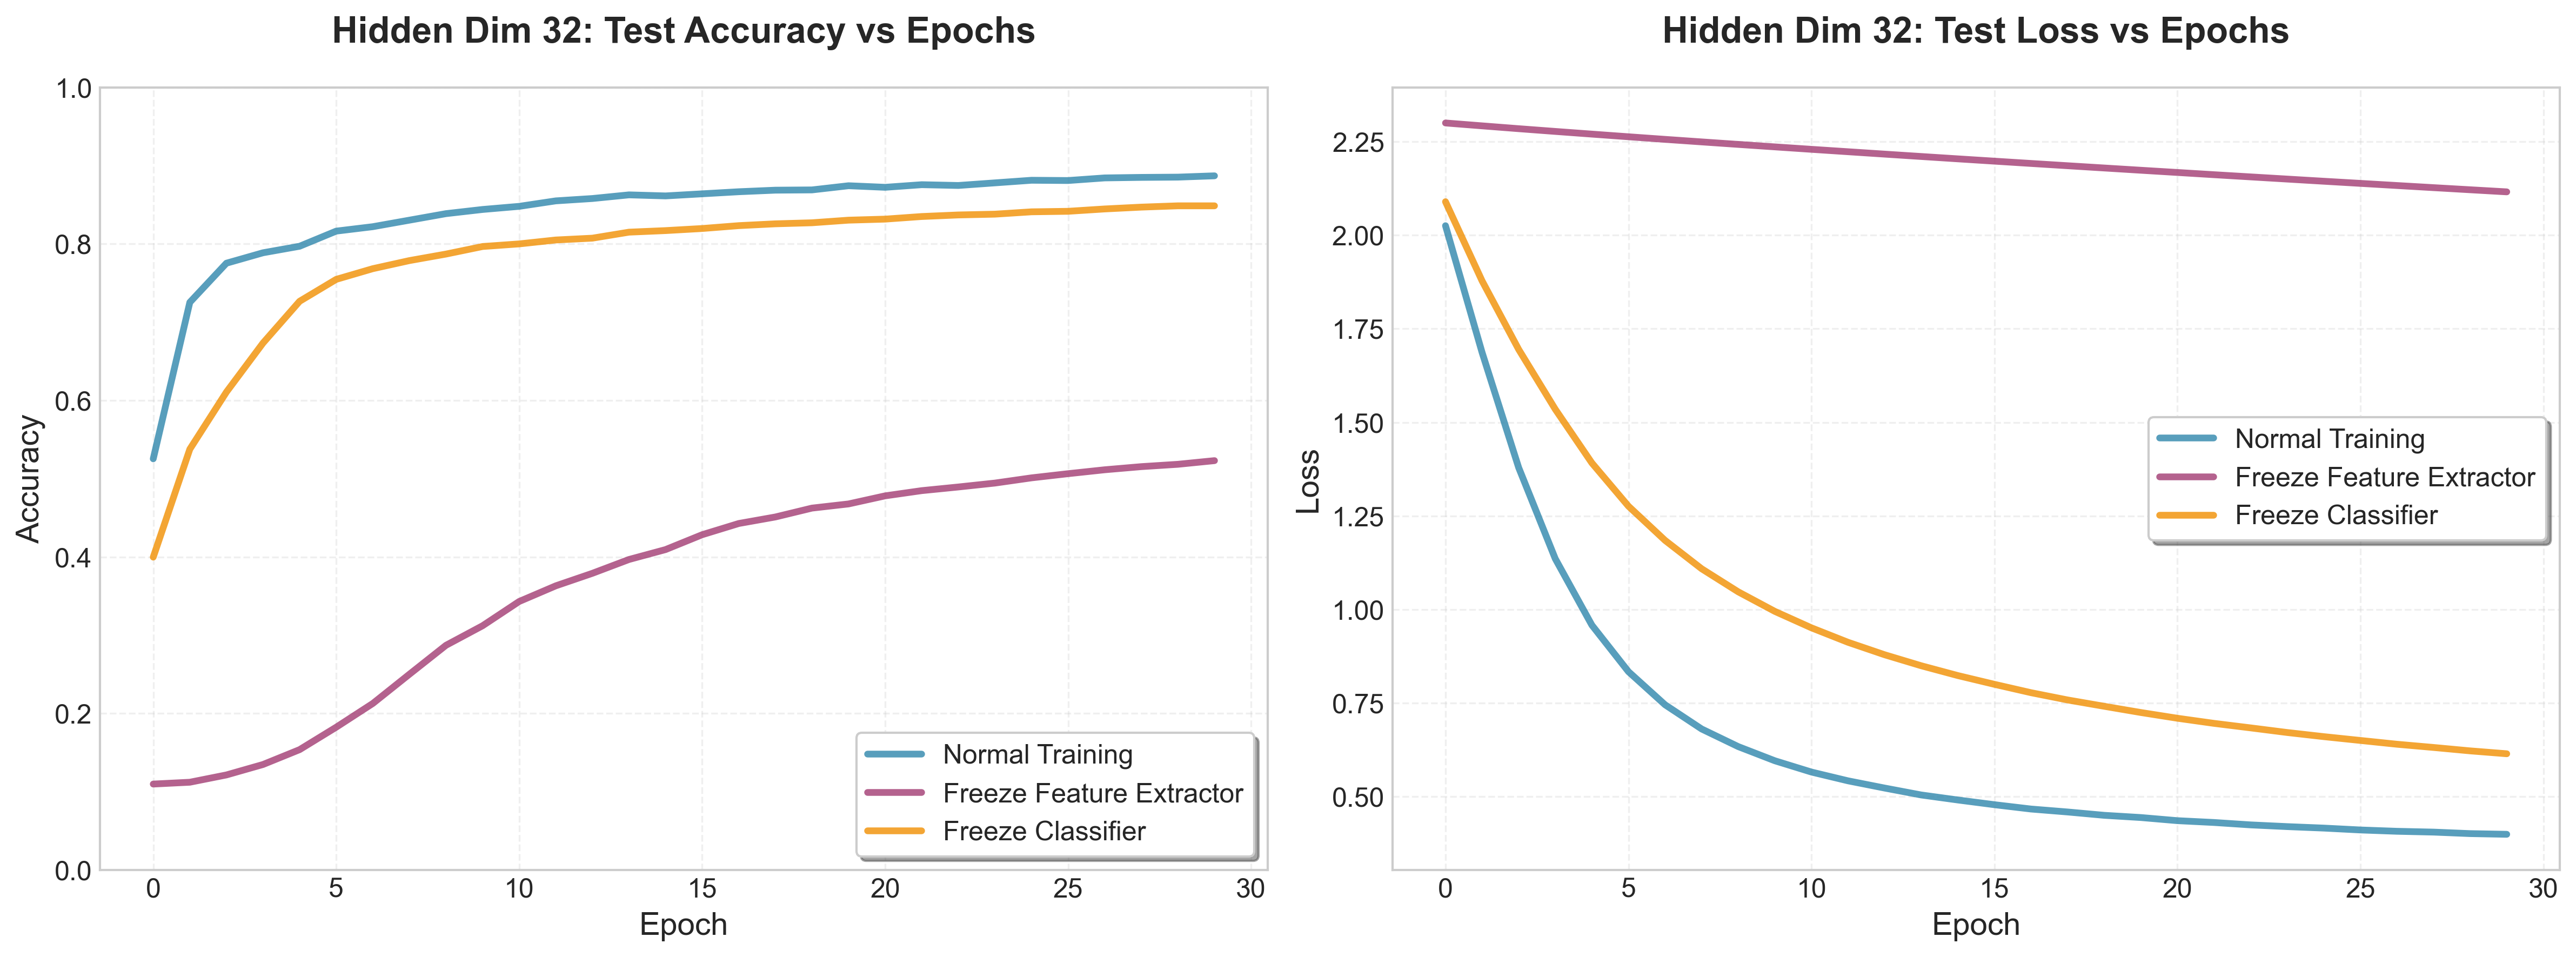
\includegraphics[width=0.8\textwidth]{../images/dd/hidden_32_comparison.png}
    \caption{冻结实验结果对比(隐藏层神经元数为32)}
    \label{fig:hidden_32_comparison.png}
\end{figure}
\begin{figure}[H]
    \centering
    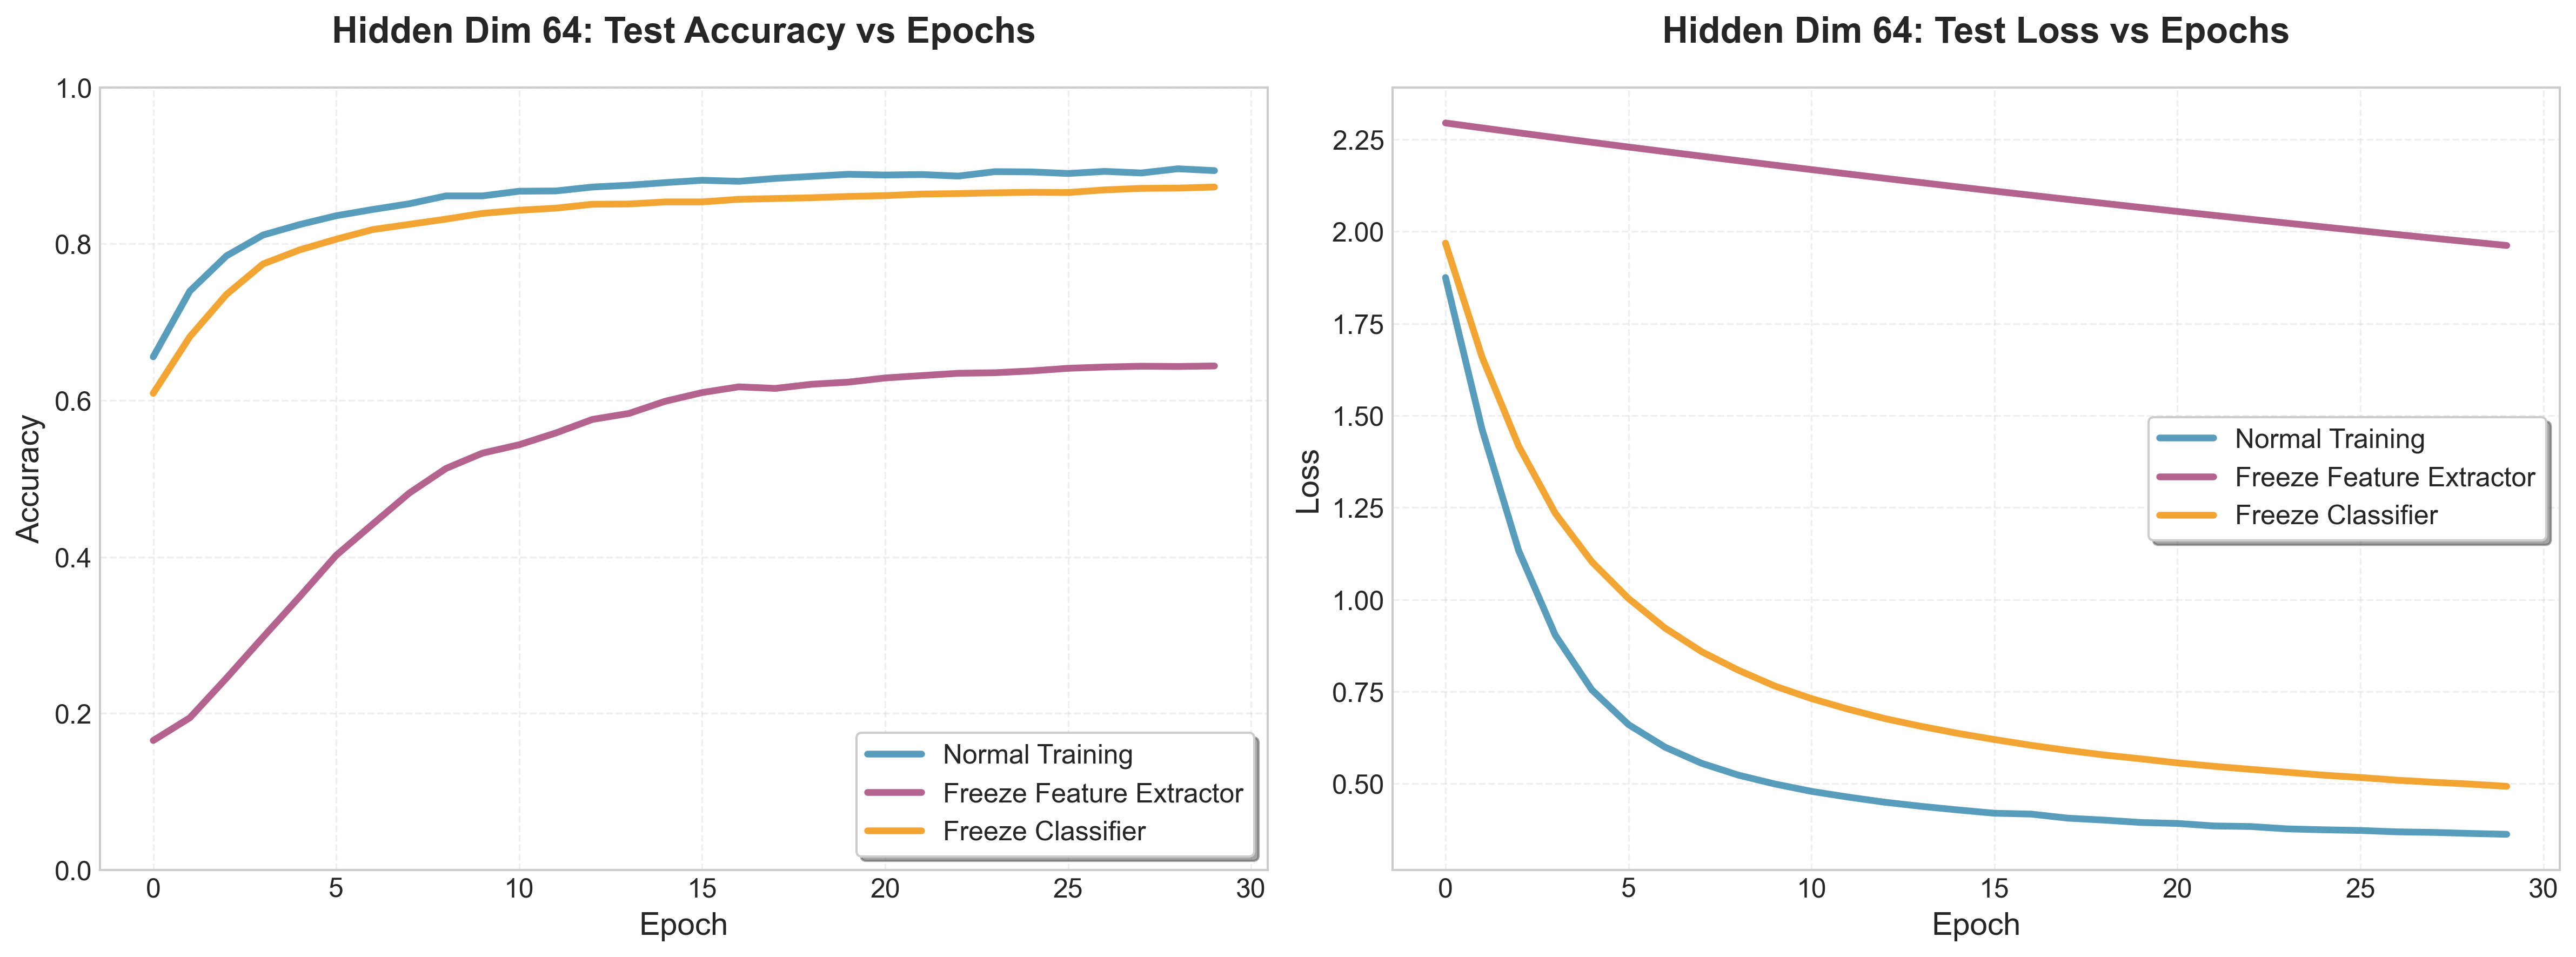
\includegraphics[width=0.8\textwidth]{../images/dd/hidden_64_comparison.png}
    \caption{冻结实验结果对比(隐藏层神经元数为64)}
    \label{fig:hidden_64_comparison.png}
\end{figure}
\begin{figure}[H]
    \centering
    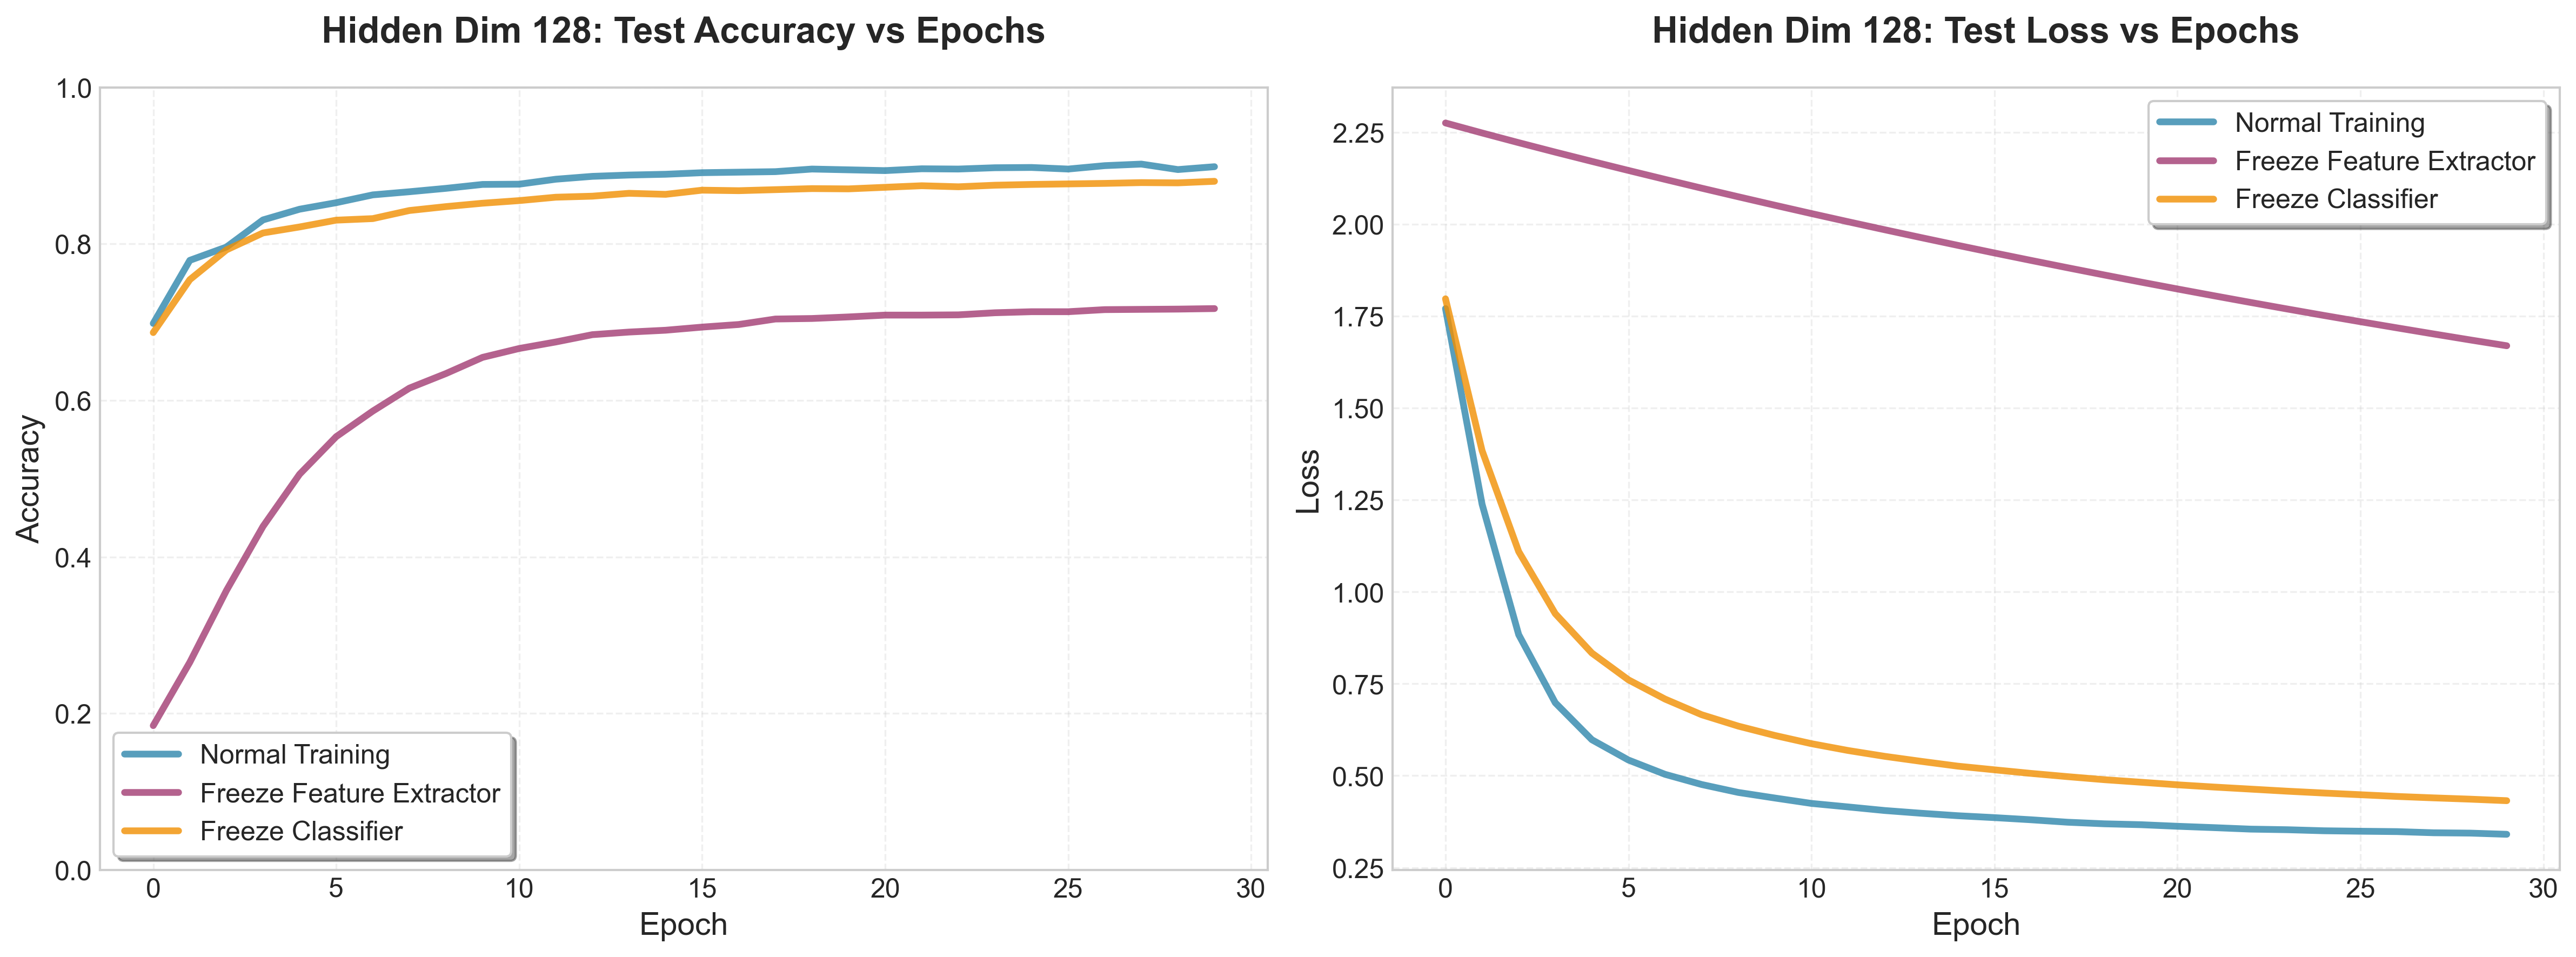
\includegraphics[width=0.8\textwidth]{../images/dd/hidden_128_comparison.png}
    \caption{冻结实验结果对比(隐藏层神经元数为128)}
    \label{fig:hidden_128_comparison.png}
\end{figure}
\begin{figure}[H]
    \centering
    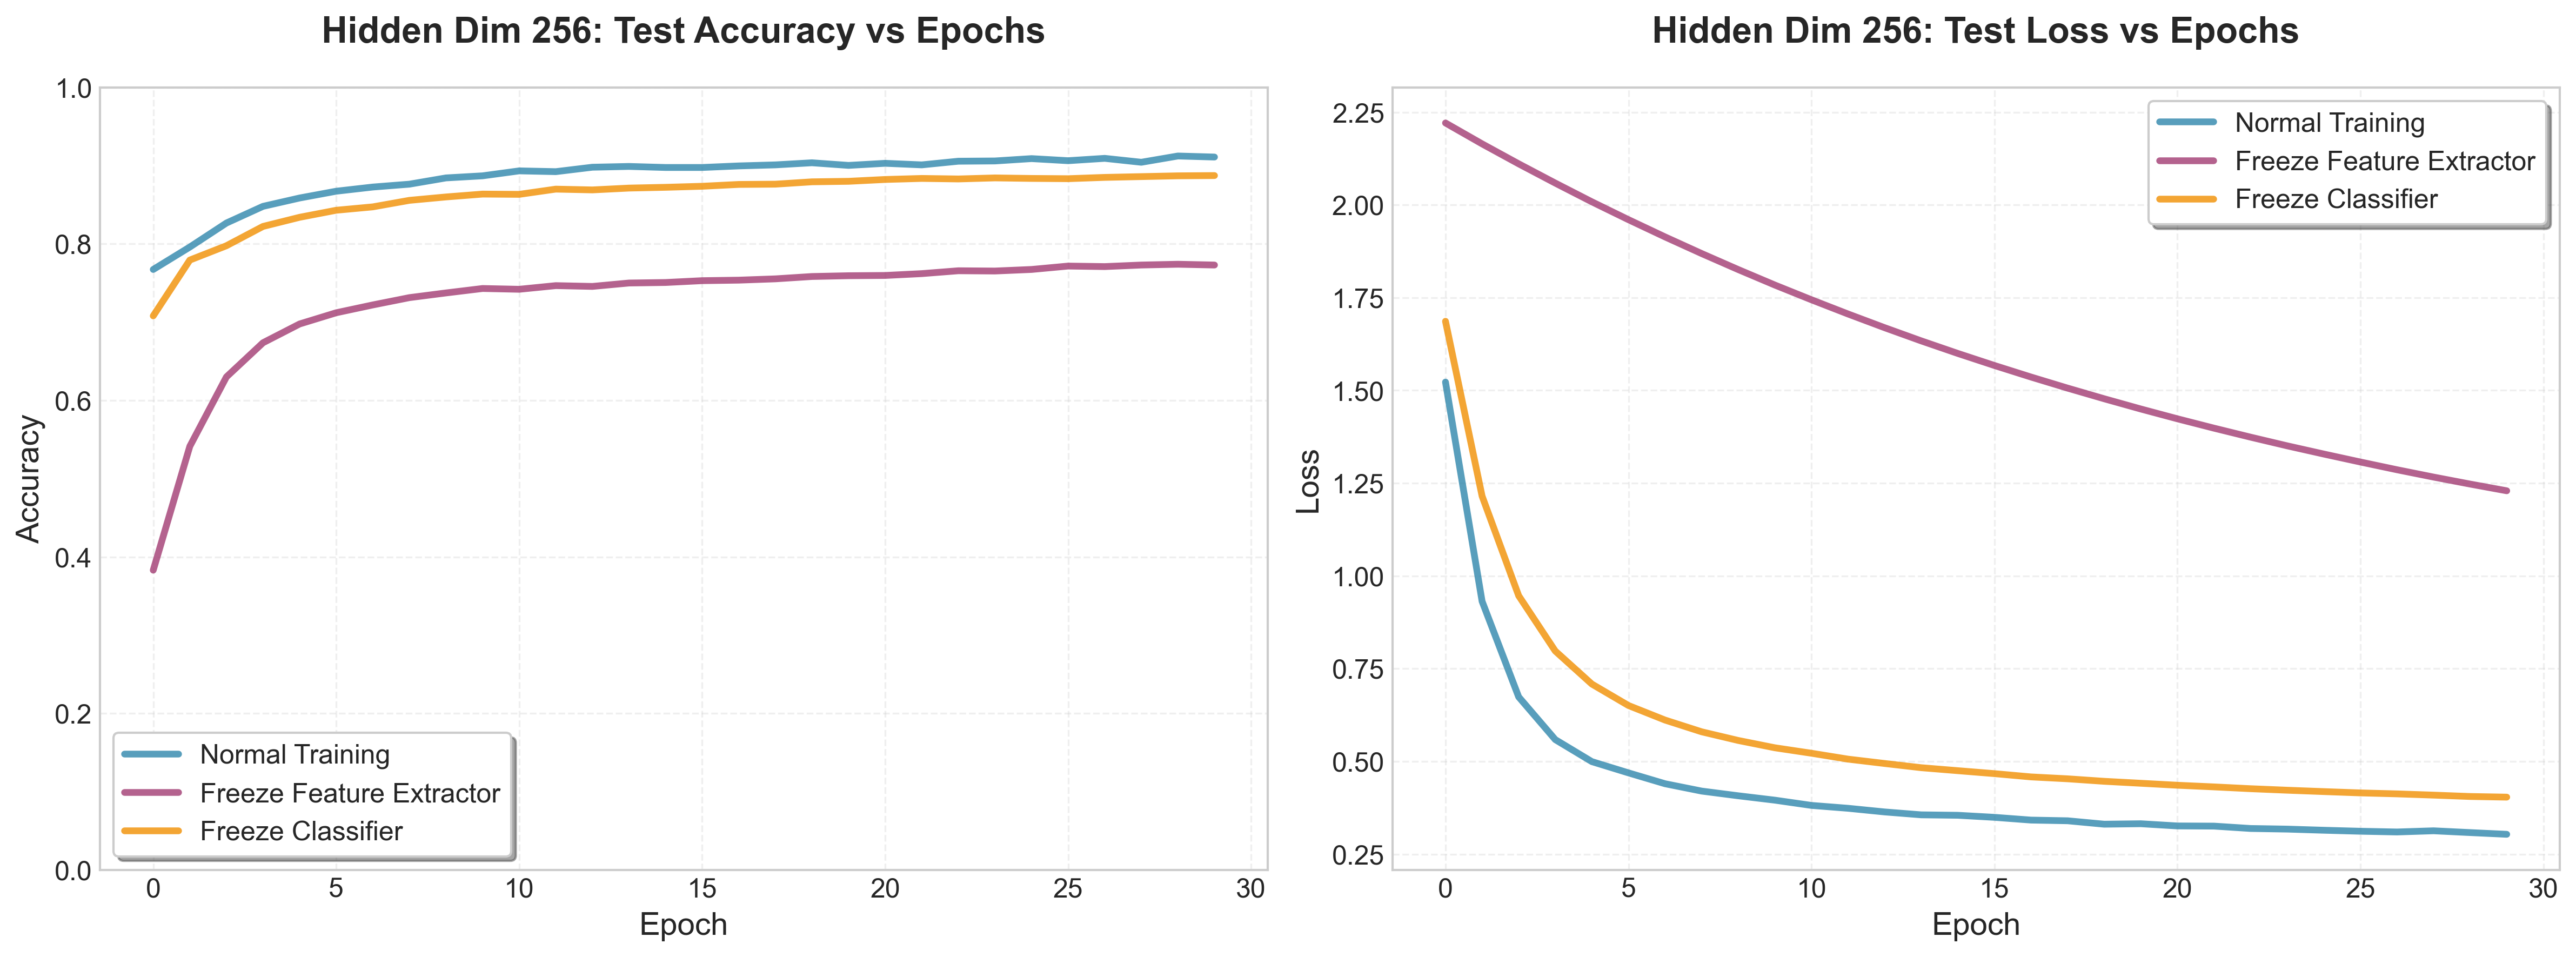
\includegraphics[width=0.8\textwidth]{../images/dd/hidden_256_comparison.png}
    \caption{冻结实验结果对比(隐藏层神经元数为256)}
    \label{fig:hidden_256_comparison.png}
\end{figure}


\section{团队分工}

本项目由五位成员共同完成,团队分工明确,协作紧密。具体任务分配如下表所示:

\begin{table}[H]
  \centering
  \caption{团队成员分工表}
  \begin{tabular}{cll}
    \toprule
    姓名 & 主要负责内容  \\\midrule
    张子路 & 实验任务设计,实验报告撰写 \\\
    郭子逸 & 手动反向传播实现、MLP/CNN结构设计  \\\
    龚正硕 & 训练曲线绘图 , MNIST统计特征提取 \\\
    康琪 & 实验报告撰写 ,数据处理与可视化分析 \\\
    魏玉涛 & 开发可视化交互组件,t-SNE 降维可视化\\\bottomrule
  \end{tabular}
  \label{tab:team-work}
\end{table}

团队成员在本项目中均积极参与,协作高效,在模型构建、实验验证、现象分析和撰写总结等方面密切配合,确保了项目的完